\chapter*{Exercises}
\phantomsection
\addcontentsline{toc}{chapter}{Exercises}
\setcounter{exercisegroup}{1}
\edef\CurrentExerciseGroup{\arabic{exercisegroup}}
\section*{\texorpdfstring{\S\CurrentExerciseGroup}{Section \CurrentExerciseGroup}}
\phantomsection
\addcontentsline{toc}{section}{\texorpdfstring{Exercises for \S\CurrentExerciseGroup}{Exercises for Section \CurrentExerciseGroup}}

\begin{enumerate}
\def\labelenumi{\arabic{enumi})}
\item
  Let E be the vector space of functions \(x \mapsto g(x) = \int_{0}^{x} f(t) dt\) defined on the interval \([0,1]\) of R, where f runs over the set of regulated functions on \([0,1]\) . Let P be the set of increasing functions belonging to E. Show that P is a convex cone such that E = P - P, \(P \cap (-P) = \{0\}\) , and that E, equipped with the order structure defined by the relation \(g - h \in P\) , is a Riesz space.
\item
  Let \(I \subset \mathbf{R}\) be a compact interval. Show that the subspace of \(\mathbf{R}^I\) formed by the restrictions to \(I\) of the polynomial functions (with real coefficients) is a directed ordered space but is not a Riesz space.
\item
  \begin{enumerate}
  \def\labelenumii{\alph{enumii})}
  \tightlist
  \item
    Let E be a Riesz space, H a linear subspace of E. If, for any pair of elements x, y of H, \(\sup(x,y)\) belongs to H, then H is said to be a co-lattice subspace. For this to be the case, it is necessary and sufficient that the relation \(x \in H\) imply \(|x| \in H\) .
  \end{enumerate}
\end{enumerate}

\begin{enumerate}
\def\labelenumi{\alph{enumi})}
\setcounter{enumi}{1}
\tightlist
\item
  Let I be a compact interval in R, H the subspace of \(R^{I}\) formed by the restrictions to I of the first-degree polynomials \(t \mapsto \alpha t + \beta\) . Show that H is not a co-lattice subspace of \(R^{I}\) but that H is a Riesz space (for the structure induced by that of \(R^{I}\) ).
\end{enumerate}

\begin{enumerate}
\def\labelenumi{\arabic{enumi})}
\setcounter{enumi}{3}
\item
  Let E be a Riesz space, H a linear subspace of E. One says that H is an isolated subspace of E if the relations \(x \in H\) , \(|y| \leqslant |x|\) imply \(y \in H\) . In this case, let P be the set of elements \(\dot{x}\) of the quotient space E/H such that there exists at least one element \(x \geqslant 0\) in the class \(\dot{x}\) . Show that P is the set of elements \(\geqslant 0\) for an order structure on E/H, compatible with the vector space structure of E/H, for which E/H is a Riesz space (cf.~A, VI, §1, Exer. 4).
\item
  \begin{enumerate}
  \def\labelenumii{\alph{enumii})}
  \tightlist
  \item
    An ordered vector space E is said to be archimedean if every \(x \in E\) such that the set of nx (n an integer \(\geqslant 0\) ) is bounded above, is necessarily \(\leqslant 0\) (A, VI, §1, Exer. 31). Show that this condition is equivalent to the following: the intersection of any plane passing through 0 with the convex cone P of elements \(\geqslant 0\) of E is a closed angular sector. Show that for an ordered vector space to be archimedean, it is necessary and sufficient that it be isomorphic to a subspace of a fully lattice-ordered space (cf.~A, VI, §1, Exer. 31).
  \end{enumerate}
\end{enumerate}

\begin{enumerate}
\def\labelenumi{\alph{enumi})}
\setcounter{enumi}{1}
\tightlist
\item
  Let F be the Riesz space \(\mathbf{R}^{\mathbf{R}}\) of real-valued functions defined on \(\mathbf{R}\) and let H be the subspace \(\mathcal{B}(\mathbf{R})\) of bounded functions on \(\mathbf{R}\) ; H is an isolated subspace of F (Exer. 4). Show that the Riesz space \(\mathrm{E} = \mathrm{F} / \mathrm{H}\) (Exer. 4) is not archimedean: more precisely, show that for every element \(x \geqslant 0\) of E, there exists a \(y \in \mathrm{E}\) such that \(y \geqslant nx\) for every integer \(n \geqslant 0\) .
\end{enumerate}

\begin{enumerate}
\def\labelenumi{\arabic{enumi})}
\setcounter{enumi}{5}
\item
  Let E be a fully lattice-ordered space, V a linear subspace of E. Show that, for there to exist in E a supplement W of V such that E is the ordered direct sum of V and W, it is necessary and sufficient that V be a band; W is then necessarily identical to the band of elements of E that are alien to every element of V.
\item
  Let E be a fully lattice-ordered space, H an isolated subspace of E (Exer. 4). If \(B_{1}\) and \(B_{2}\) are two supplementary bands in E, show that H is the ordered direct sum of \(H_{1}=H\cap B_{1}\) and \(H_{2}=H\cap B_{2}\) , and that the Riesz space E/H is the ordered direct sum of the Riesz spaces \(B_{1}/H_{1}\) and \(B_{2}/H_{2}\) .
\item
  Let \((\mathbf{E}_{\iota})\) be a family of fully lattice-ordered spaces, E the product space of the \(E_{\iota}\) (which is fully lattice-ordered). Show that if B is a band in E, then each of its projections \(\mathrm{B}_{\iota} = \mathrm{pr}_{\iota}(\mathrm{B})\) is a band in \(E_{\iota}\) , and B is identical to the product of the \(B_{\iota}\) . From this, deduce the determination of the bands in the space \(R^{A}\) of mappings of a set A into R. Show that, in the space \(\mathcal{B}(A)\) of bounded real-valued functions on A, every band is the trace on \(\mathcal{B}(A)\) of a band in \(R^{A}\) .
\item
  Let E be a fully lattice-ordered space. A filter \(\mathfrak{F}\) on E is said to be bounded above (resp. bounded below, bounded) if there is a set in \(\mathfrak{F}\) that is bounded above (resp. bounded below, bounded). For a filter \(\mathfrak{F}\) that is bounded above (resp. below), the limit superior (resp. limit inferior) of \(\mathfrak{F}\) , denoted lim sup \(\mathfrak{F}\) (resp. lim inf \(\mathfrak{F}\) ) is defined to be the element \(\inf_{\mathrm{X}}(\sup \mathrm{X})\) (resp. \(\sup_{\mathrm{X}}(\inf \mathrm{X})\) ) of E, where X runs over the set of sets
\end{enumerate}

in \(\mathfrak{F}\) that are bounded above (resp. bounded below). If \(\mathfrak{F}\) is bounded, then \(\liminf\mathfrak{F} \leqslant \limsup\mathfrak{F}\) ; \(\mathfrak{F}\) is said to have a limit, or to be convergent, for the order structure of E, if \(\limsup\mathfrak{F} = \liminf\mathfrak{F}\) ; the common value of these two elements is then denoted \(\lim\mathfrak{F}\) , and \(\mathfrak{F}\) is said to converge to this element of E. If a bounded filter has a limit, then every finer filter has the same limit (for the order structure).

\begin{enumerate}
\def\labelenumi{\alph{enumi})}
\tightlist
\item
  In order that a bounded filter \(\mathfrak{F}\) have a limit for the order structure, it is necessary and sufficient that \(\inf_{\mathbf{X}} (\sup \mathbf{X} - \inf \mathbf{X}) = 0\) as \(\mathbf{X}\) runs over the set of bounded elements of \(\mathfrak{F}\) (one can make use of the fact that if, in E, \((x_{\alpha})\) and \((y_{\alpha})\) are two decreasing families that are bounded below, having the same right-directed index set, then
\end{enumerate}

\[
\inf (x _ {\alpha} + y _ {\alpha}) = \inf x _ {\alpha} + \inf y _ {\alpha};
\]

to prove this formula, one observes that \(\inf (x_{\alpha} + y_{\alpha})\leqslant x_{\beta} + y_{\gamma}\) for every pair of indices \(\beta ,\gamma)\) .

\begin{enumerate}
\def\labelenumi{\alph{enumi})}
\setcounter{enumi}{1}
\item
  Let A be a set filtered by a filter G, f a mapping of A into E; f is said to have a limit with respect to G for the order structure of E if \(f(\mathfrak{G})\) is a base of a bounded filter having a limit in E (for the order structure). Show that if A is a directed ordered set and f is an increasing mapping of A into E that is bounded above on A, then f has a limit with respect to the section filter of A, equal to \(\sup f(x)\) .
\item
  Let \((\mathbf{E}_{\iota})\) be a family of fully lattice-ordered spaces, E the product fully lattice-ordered space of the \(E_{\iota}\) . In order that a bounded filter F on E be convergent for the order structure, it is necessary and sufficient that, for every \(\iota\) , the filter with base \(\Pr_{\iota}(\mathfrak{F})\) be convergent in \(E_{\iota}\) ; if \(a_{\iota}\) is its limit, then \(a = (a_{\iota})\) is the limit of F.
\end{enumerate}

¶ 10) a) Let E be a fully lattice-ordered space; there exists a topology \(\mathcal{T}_0(E)\) on E that is the finest of the topologies \(\mathcal{T}\) on E for which every bounded filter \(\mathfrak{F}\) on E that converges in the sense of the order structure (Exer. 9) converges to the same limit for \(\mathcal{T}\) .

Let E and F be two fully lattice-ordered spaces, f a mapping of E into F such that, for every bounded filter F on E that is convergent for the order structure, \(f(\mathfrak{F})\) is a base of a bounded filter on F that converges to \(f(\lim \mathfrak{F})\) for the order structure. Show that, under these conditions, f is continuous for the topologies \(\mathcal{T}_{0}(\mathrm{E})\) and \(\mathcal{T}_{0}(\mathrm{F})\) .

\begin{enumerate}
\def\labelenumi{\alph{enumi})}
\setcounter{enumi}{1}
\item
  Deduce from a) that the topology \(\mathcal{T}_{0}(\mathrm{E})\) is compatible with the vector space structure of E and that the mapping \(x \mapsto |x|\) is continuous for this topology. Prove that \(\mathcal{T}_{0}(\mathrm{E})\) is compatible with the ordered vector space structure of E and, from this, deduce that this topology is Hausdorff.
\item
  Given any infinite set A, let \(\mathrm{E} = \mathcal{B}(\mathrm{A})\) be the fully lattice-ordered space of bounded real-valued functions on A. Let \(\Phi\) be the set of numerical functions \(\varphi\) (finite or not) defined on A such that \(\varphi(t) > 0\) for all \(t \in A\) and such that, for every integer n \textgreater{} 0, the set of \(t \in A\) such that \(\varphi(t) \leqslant n\) is finite. For every function \(\varphi \in \Phi\) , let \(V_{\varphi}\) be the set of \(x \in E\) such that \(|x| \leqslant \varphi\) ; show that the sets \(V_{\varphi}\) form a fundamental system of neighborhoods of 0 for a topology \(\mathcal{T}_{1}(\mathrm{E})\) compatible with the ordered vector space structure of E, and for which E is Hausdorff and complete. Show that the topology \(\mathcal{T}_{0}(\mathrm{E})\) is finer than \(\mathcal{T}_{1}(\mathrm{E})\) , but strictly coarser than the topology of uniform convergence in A (defined by the norm \(\|x\| = \sup_{t \in A} |x(t)|\) ) (consider the elements \(1 - \varphi_{X}\) of \(\mathcal{B}(\mathrm{A})\) ,
\end{enumerate}

where X runs over the set of finite subsets of A, \(\varphi_{X}\) being the characteristic function of X). Deduce from this that in order for a subset of E to be bounded (for the order structure), it is necessary and sufficient that it be bounded for the topology \(\mathcal{T}_{0}(E)\) (TVS, III, §1, No.~2). Show that every filter on E that is bounded and convergent for the topology \(\mathcal{T}_{0}(E)\) is convergent to the same limit for the order structure. Finally, show that there exist filters on E that are convergent for \(\mathcal{T}_{0}(E)\) but are not bounded.

¶ 11) Let E be a fully lattice-ordered space, \((x_{\iota})_{\iota \in I}\) a family of elements of E. For every finite subset H of I, set \(s_{H} = \sum_{\iota \in H} x_{\iota}\) ; the family \((x_{\iota})_{\iota \in I}\) is said to be summable

for the order structure of E if the mapping \(\mathrm{H} \mapsto s_{\mathrm{H}}\) has a limit for this order structure, with respect to the directed ordered set \(\mathfrak{F}(\mathrm{I})\) of finite subsets of I; this limit \(s\) is then called the sum of the family \((x_{\iota})_{\iota \in \mathrm{I}}\) and is denoted \(\sum_{\iota \in \mathrm{I}} x_{\iota}\) .

\begin{enumerate}
\def\labelenumi{\alph{enumi})}
\item
  For a family \((x_{\iota})_{\iota \in I}\) to be summable, it is necessary and sufficient that: \(1^{\circ}\) for every finite subset H of I, the set of \(|s_{K}|\) , where K runs over the set of finite subsets of I that do not intersect H, has a supremum \(r_{\mathrm{H}}\) in E; \(2^{\circ} \inf_{\mathrm{H}} r_{\mathrm{H}} = 0\) as H runs over \(\mathfrak{F}(I)\) (make use of Exer. 9 a)).
\item
  Generalize to summable families, for the order structure of E, the properties of summable families in commutative topological groups (GT, III, §5, Props. 2, 3 and Th. 2).
\item
  Let \((x_{\iota})_{\iota \in I}\) be a family of elements \(\geqslant 0\) of E; for the family to be summable, it is necessary and sufficient that the set of finite partial sums \(s_{\mathrm{H}}\) be bounded above (make use of Exer. 9 b)). If \((x_{\iota})_{\iota \in I}\) is summable and if \((y_{\iota})_{\iota \in I}\) is a family of elements such that \(0 \leqslant y_{\iota} \leqslant x_{\iota}\) for all \(\iota\) , show that the family \((y_{\iota})\) is summable and that \(\sum_{\iota \in I} y_{\iota} \leqslant \sum_{\iota \in I} x_{\iota}\) , with equality holding only if \(x_{\iota} = y_{\iota}\) for all \(\iota \in I\) .
\item
  Let \((x_{\iota})\) be a family of elements of E; show that if the family \((|x_{\iota}|)\) is summable for the order structure, then so is the family \((x_{\iota})\) .
\end{enumerate}

\begin{enumerate}
\def\labelenumi{\arabic{enumi})}
\setcounter{enumi}{11}
\tightlist
\item
  Let \(\mathbf{E}\) be a fully lattice-ordered space. Show that there exists a family \((u_{\iota})\) of elements \(> 0\) of \(\mathbf{E}\) such that \(u_{\iota}\) and \(u_{\kappa}\) are alien for every pair of distinct indices \(\iota, \kappa\) , and such that for every \(x > 0\) in \(\mathbf{E}\) there exists at least one index \(\iota\) such that \(\inf(x, u_{\iota}) > 0\) (use Zorn's lemma). From this, deduce that for every \(x \geqslant 0\) there exists one and only one family \((x_{\iota})\) of elements \(\geqslant 0\) of \(\mathbf{E}\) such that, for every \(\iota, x_{\iota}\) belongs to the band \(B_{\iota}\) generated by \(u_{\iota}\) , and such that \(x = \sum_{\iota} x_{\iota}\) for the order structure of \(\mathbf{E}\) .
\end{enumerate}

(take \(x_{\iota}\) to be the component of \(x\) in the band \(B_{\iota}\) ). Conversely, every family \((x_{\iota})\) of elements \(\geqslant 0\) of E that is bounded above, such that \(x_{\iota} \in B_{\iota}\) for all \(\iota\) , is summable in E (Exer. 11).

¶ 13 a) Let E be a fully lattice-ordered space. If \(u \neq 0\) is an arbitrary element of E, show that the set of \(x \in E\) such that there exists an integer \(n\) for which \(|x| \leqslant n|u|\) , is a linear subspace \(C_u\) that is a fully lattice-ordered and co-lattice subspace (Exer. 3) of E. For every \(x \in C_u\) , one denotes by \(\|x\|\) the infimum of the scalars \(\lambda > 0\) such that \(|x| \leqslant \lambda |u|\) ; show that \(\|x\|\) is a norm on \(C_u\) (make use of the fact that E is archimedean (Exer. 5)), that \(C_u\) , equipped with this norm, is complete, and that \(\|x\| = \sup(\|x^+\|, \|x^-\|)\) .

\begin{enumerate}
\def\labelenumi{\alph{enumi})}
\setcounter{enumi}{1}
\item
  Let \(\mathcal{I}\) be the set of components of \(u\) in the bands of the space \(\mathrm{C}_u\) ; show that \(\mathcal{I}\) is the set of elements \(c\) of \(\mathrm{C}_u\) such that \(0 \leqslant c \leqslant u\) and \(\inf(c, u - c) = 0\) (use Riesz's theorem). Show that \(\mathcal{I}\) is closed in the normed space \(\mathrm{C}_u\) and that, for the order relation induced by that of \(\mathrm{C}_u\) , \(\mathcal{I}\) is a complete Boolean algebra (S, III, §1, Exers. 11 and 17; it suffices to show that if \((c_\iota)\) is a family of elements of \(\mathcal{I}\) then \(\sup_{\iota} c_\iota\) belongs to \(\mathcal{I}\) ).
\item
  Let \(x\) be any element of \(\mathbf{C}_u\) ; for every \(\lambda \in \mathbf{R}\) let \(c(\lambda)\) be the component of \(u\) in the band of \(\mathbf{C}_u\) generated by \((\lambda u - x)^+\) . Show that if \(\lambda \leqslant \mu\) then \(c(\lambda) \leqslant c(\mu)\) ; \(c(\lambda) = 0\) for \(\lambda < -\|x\|\) , and \(c(\lambda) = u\) for \(\lambda > \|x\|\) . Show that if \(c \in \mathcal{I}\) is such that \(c \leqslant c(\lambda)\) , then the component of \(x\) in the band generated by \(c\) is \(\leqslant \lambda c\) (observe that the bands generated by \(c(\lambda)\) and by \((\lambda u - x)^+\) are identical, and that the component of \(\lambda u - x\) in this band is equal to that of \((\lambda u - x)^+\) ; from this, deduce that the component of \(x\) in this same band is \(\leqslant \lambda c(\lambda)\) ). Similarly, show that if \(c \in \mathcal{I}\) is such that \(c \leqslant u - c(\lambda)\) , then the component of \(x\) in the band generated by \(c\) is \(\geqslant \lambda c\) .
\item
  It is known (GT, II, §4, Exer. 12) that there exists an order structure isomorphism \(c \mapsto \theta_c\) of the Boolean algebra \(\mathcal{I}\) onto the Boolean algebra formed by the characteristic functions of the sets in a compact, totally disconnected space S that are both open and closed. Show that the relation \(\sum_{i} \lambda_i c_i = 0\) implies that the function \(\sum_{i} \lambda_i \theta_{c_i}\) is 0 on S (make use of the decomposition lemma); deduce from this remark and c) that the mapping \(c \mapsto \theta_{c}\) may be extended to an isomorphism \(x \mapsto \theta_{x}\) of the normed space \(C_{u}\) onto the normed space \(\mathcal{C}(\mathrm{S};\mathbf{R})\) of continuous real-valued functions on S, so that \((\theta_{x})^{+} = \theta_{x^{+}}\) . (With the help of c), show that for every \(x \in C_{u}\) and every \(\varepsilon > 0\) , there exists an increasing sequence \((\lambda_{i})_{0 \leqslant i \leqslant n}\) of real numbers such that \(\lambda_{i} - \lambda_{i-1} \leqslant \varepsilon\)
\end{enumerate}

and \(0 \leqslant x - \sum_{i=1}^{n} \lambda_{i-1} (c(\lambda_{i-1}) - c(\lambda_i)) \leqslant \varepsilon u\) .

\begin{enumerate}
\def\labelenumi{\alph{enumi})}
\setcounter{enumi}{4}
\item
  In order that S be finite, it is necessary and sufficient that \(C_{u}\) be finite-dimensional; from this, deduce (with the help of Exer. 12) that every finite-dimensional fully lattice-ordered space is isomorphic to a product space \(R^{n}\) (cf.~§2, Exer. 7).
\item
  Show that S is an extremely disconnected space (GT, I, §11, Exer. 21) (make use of the fact that \(\mathcal{I}\) is a complete Boolean algebra). An extremely disconnected compact space is called a Stone space. Show that if X is a Stone space then, for every lower semi-continuous numerical function \(f\) on X, the upper semi-continuous regularization \(g\) of \(f\) (GT, IV, §6, No.~2) is continuous (for every \(a < g(x)\) show that \(x\) cannot belong to the closure of the (open) set of \(y\) such that \(g(y) < a\) , by observing that \(f(z) \leqslant a\) at a point \(z\) in the closure of this set). From this, deduce that \(\mathcal{C}(\mathrm{X};\mathbf{R})\) is then a fully lattice-ordered space. Show that when the Stone space X is infinite, the supremum in \(\mathcal{C}(\mathrm{X};\mathbf{R})\) of a set that is bounded above is not necessarily equal to its upper envelope (consider a non-closed open set in X); however, these two functions are equal on the complement of a meager set (consider the set of points where their difference is \(\geqslant 1/n\) ).
\item
  Let X be a Stone space; show that if f is a bounded real-valued function, defined on the complement of a nowhere dense subset M of X and continuous on X - M, then \(f\) may be extended by continuity to all of X (make use of the fact that \(\mathcal{C}(X; \mathbf{R})\) is fully lattice-ordered). From this, deduce that the set \(\mathcal{Q}(X; \overline{\mathbf{R}})\) , of continuous numerical functions \(f\) on X (finite or not) such that \(f(+\infty)\) and \(f(-\infty)\) are nowhere dense in X, is a fully lattice-ordered vector space.
\item
  Show that the band \(B_{u}\) generated by u in E is isomorphic (as an ordered space) to an isolated subspace (Exer. 4) of \(\mathcal{Q}(\mathrm{X};\overline{\mathbf{R}})\) (regard an element \(f \geqslant 0\) of \(\mathcal{Q}(\mathrm{X};\overline{\mathbf{R}})\) as the supremum of the elements \(\inf(f,n)\) ).
\end{enumerate}

\begin{enumerate}
\def\labelenumi{\arabic{enumi})}
\setcounter{enumi}{13}
\tightlist
\item
  Let E be a Riesz space, equipped with a Hausdorff topology compatible with the ordered vector space structure of E.
\end{enumerate}

\begin{enumerate}
\def\labelenumi{\alph{enumi})}
\item
  Let K be a compact subset of E, H a subset of K that is directed for the relation \(\leqslant\) ; show that the section filter F of H is convergent. (First prove that the set L of upper bounds of H belonging to K is nonempty and compact, then that the set of cluster points of F is contained in L, and finally that there cannot exist two distinct cluster points.)
\item
  Deduce from \(a\) ) that if, in \(\mathbf{E}\) , every interval \([a,b]\) is compact, then \(\mathbf{E}\) is fully lattice-ordered.
\end{enumerate}

\setcounter{exercisegroup}{2}
\edef\CurrentExerciseGroup{\arabic{exercisegroup}}
\section*{\texorpdfstring{\S\CurrentExerciseGroup}{Section \CurrentExerciseGroup}}
\phantomsection
\addcontentsline{toc}{section}{\texorpdfstring{Exercises for \S\CurrentExerciseGroup}{Exercises for Section \CurrentExerciseGroup}}

\begin{enumerate}
\def\labelenumi{\arabic{enumi})}
\tightlist
\item
  Let E be a Riesz space, x an element \textgreater0 of E. If there exists a relatively bounded linear form L on E such that \(L(x) \neq 0\) , show that the set of nx (n an integer \textgreater0) cannot be bounded above in E. In particular, show that there does not exist any relatively bounded linear form on the Riesz space E defined in Exer. 5 b) of §1.
\end{enumerate}

¶ 2) a) Let L be a positive linear form on the Riesz space E. Consider an element a \textgreater{} 0 of E and the set of positive linear forms \(M \leqslant L\) such that: \(1^{\circ} M(x) = L(x)\) for every x such that \(0 \leqslant x \leqslant a\) ; \(2^{\circ} M(x) = 0\) for every \(x \geqslant 0\) alien to a. Show that this set of positive linear forms has a largest element \(L_{a}\) and that, for every \(x \geqslant 0\) , \(L_{a}(x) = \inf L(y)\) , where y runs over the set of all elements such that \(0 \leqslant y \leqslant x\) and x - y is alien to a. Show that \(L_{\lambda a} = L_{a}\) for every scalar \(\lambda > 0\) , and that if a and b are alien then \(L_{a+b} \leqslant L_{a} + L_{b}\) . If E is fully lattice-ordered, show that if a and b are alien in E then \(L_{a+b} = L_{a} + L_{b}\) .

\begin{enumerate}
\def\labelenumi{\alph{enumi})}
\setcounter{enumi}{1}
\tightlist
\item
  Take E to be the Riesz space of continuous real-valued functions on the interval \(\mathbf{I} = [0,1]\) of \(\mathbf{R}\) , and \(L(x) = x\left(\frac{1}{2}\right)\) ; show by means of an example that one can have \(L_{a + b} < L_a + L_b\) for two alien elements \(a, b\) of \(\mathbf{E}\) .
\end{enumerate}

\begin{enumerate}
\def\labelenumi{\arabic{enumi})}
\setcounter{enumi}{2}
\tightlist
\item
  Let \(\mathbf{E}\) be a fully lattice-ordered space.
\end{enumerate}

\begin{enumerate}
\def\labelenumi{\alph{enumi})}
\item
  Show that every linear form \(L\) on \(\mathbf{E}\) that is continuous for the topology \(\mathcal{T}_0(\mathbf{E})\) (§1, Exer. 10) is relatively bounded, and that \(|L|\) is continuous for \(\mathcal{T}_0(\mathbf{E})\) (argue by contradiction, on observing that for every \(x \in \mathbf{E}\) the sequence of elements \(x / n\) tends to 0 as \(n\) tends to infinity, for the topology \(\mathcal{T}_0(\mathbf{E})\) ).
\item
  Let A be any infinite set, U an ultrafilter on A whose sets have empty intersection. On the fully lattice-ordered space \(E = \mathcal{B}(A)\) , consider the positive linear form \(x \mapsto \lim_{\mu} x(t)\) ; show that this linear form is not continuous for the topology \(\mathcal{T}_{0}(E)\) .
\end{enumerate}

\begin{enumerate}
\def\labelenumi{\arabic{enumi})}
\setcounter{enumi}{3}
\tightlist
\item
  Let E be a fully lattice-ordered space.
\end{enumerate}

\begin{enumerate}
\def\labelenumi{\alph{enumi})}
\item
  Let \(L\) be a positive linear form on \(\mathbf{E}\) , continuous for the topology \(\mathcal{T}_0(\mathbf{E})\) (§1, Exer. 10). Show that the set of \(x \in \mathbf{E}\) such that \(L(|x|) = 0\) is a band \(Z(L)\) . Let \(S(L)\) be the band supplementary to \(Z(L)\) in \(\mathbf{E}\) (§1, Exer. 6).
\item
  Let L and M be two positive linear forms on E, continuous for \(\mathcal{T}_{0}(\mathrm{E})\) . In order that, in the space \(\Omega\) of relatively bounded linear forms on E, M belong to the band generated by L, it is necessary and sufficient that \(S(M) \subset S(L)\) . (To see that the condition is sufficient, argue by contradiction, on supposing that M does not verify the condition of Prop. 5; consider a sequence \((y_{n})\) of elements of E such that \(0 \leqslant y_{n} \leqslant x\) ,
\end{enumerate}

\(L(y_{n}) \leqslant 1 / 2^{n}\) and \(M(y_{n}) \geqslant \alpha > 0\) , and infer the existence of an element \(z \geqslant 0\) in E such that \(L(z) = 0\) and \(M(z) \geqslant \alpha\) .

\begin{enumerate}
\def\labelenumi{\alph{enumi})}
\setcounter{enumi}{2}
\tightlist
\item
  Let \(L\) and \(M\) be two positive linear forms on \(\mathbf{E}\) , continuous for \(\mathcal{T}_0(\mathbf{E})\) . In order that, in \(\Omega\) , \(L\) and \(M\) be alien, it is necessary and sufficient that \(S(L) \cap S(M) = \{0\}\) . (To see that the condition is necessary, prove that if \(S(L) \cap S(M)\) does not reduce to 0 then the bands in \(\Omega\) generated by \(L\) and \(M\) have an element \(\neq 0\) in common, by using b).)
\end{enumerate}

¶ 5) a) Let E be a Riesz space, H an isolated linear subspace of E (§1, Exer. 4). Let Ω be the space of relatively bounded linear forms on E and let Θ be the subspace of Ω consisting of the linear forms \(L \in \Omega\) that are zero on H. Show that Θ is an isolated subspace of Ω and that Θ is a fully lattice-ordered space isomorphic to the space of relatively bounded linear forms on the Riesz space E/H.

\begin{enumerate}
\def\labelenumi{\alph{enumi})}
\setcounter{enumi}{1}
\tightlist
\item
  For a linear mapping \(u\) of \(E\) into a Riesz space \(F\) , the following conditions are equivalent:
\end{enumerate}

\(\alpha) u(\sup(x, y)) = \sup(u(x), u(y));\)

\(\beta) u(\inf(x, y)) = \inf(u(x), u(y));\)

\(\gamma) u(x^{+}) = (u(x))^{+}\) ;

\(\delta)\) the relation \(\inf (x,y) = 0\) implies \(\inf (u(x),u(y)) = 0\)

One then says that u is a latticial linear mapping.

\begin{enumerate}
\def\labelenumi{\alph{enumi})}
\setcounter{enumi}{2}
\item
  For a linear subspace H of E to be maximal in the set of isolated subspaces \(\neq\) E, it is necessary and sufficient that it be of the form \(\operatorname{Ker}(f)\) , where \(f\) is a latticial linear form \(\neq 0\) . (Make use of GT, V, §3, Exer. 1.)
\item
  Give an example of a Riesz space not reduced to 0 that contains no maximal isolated subspace (cf.~§1, Exer. 5 b)).
\end{enumerate}

¶ 6) Let E be a Riesz space, Ω the fully lattice-ordered space of relatively bounded linear forms on E, and F a co-lattice subspace of Ω (§1, Exer. 3). For every \(x \in E\) , the mapping \(x' \mapsto \langle x, x' \rangle\) of F into R is a relatively bounded linear form \(u_x\) on F, and the mapping \(x \mapsto u_x\) is an increasing linear mapping of E into the fully lattice-ordered space Ω' of relatively bounded linear forms on F. In order that \(x \mapsto u_x\) be an isomorphism of E onto a co-lattice subspace of Ω', that is, for \(u_x > 0\) to imply x \textgreater{} 0, and that \(u_{\text{sup}(x,y)} = \text{sup}(u_x, u_y)\) , it is necessary and sufficient that the following two conditions be verified: 1° for every x \textgreater{} 0 in E, there exists an \(x' > 0\) in F such that \(\langle x, x' \rangle > 0\) ; 2° for every pair of alien elements \(y \geqslant 0\) , \(z \geqslant 0\) of E, for every number \(\varepsilon > 0\) and for every \(x' \geqslant 0\) in F, there exist two elements \(y' \geqslant 0\) , \(z' \geqslant 0\) of F such that \(x' = y' + z'\) and \(\langle y, y' \rangle + \langle z, z' \rangle \leqslant \varepsilon\) . (Observe that if the second condition is verified and if v is a positive linear form on F such that \(v \geqslant u_x\) , then \(v(x') \geqslant \langle x^+, x' \rangle - \varepsilon\) for every \(x' \geqslant 0\) in F and every \(\varepsilon > 0\) .)

If the condition \(2^{\circ}\) is fulfilled but not condition \(1^{\circ}\) , then the set of \(x \in E\) such that \(\langle x, x' \rangle = 0\) for all \(x' \in F\) is an isolated linear subspace \(H\) of \(E\) . By passage to the quotient, the mapping \(x \mapsto u_x\) then defines an isomorphism of the Riesz space \(E / H\) onto a co-lattice subspace of \(\Omega'\) .

Show that when \(\mathbf{F} = \Omega\) , the above condition \(2^{\circ}\) is always verified (make use of Exer. 2).

\begin{enumerate}
\def\labelenumi{\arabic{enumi})}
\setcounter{enumi}{6}
\tightlist
\item
  Let \(E\) be a Riesz space of finite dimension \(n\) .
\end{enumerate}

\begin{enumerate}
\def\labelenumi{\alph{enumi})}
\item
  If E is archimedean (§1, Exer. 5), show that the cone P of elements \(\geqslant 0\) of E is closed and has an interior point. From this, deduce that the intersection of the support hyperplanes of P reduces to 0 (make use of the fact that \(P \cap (-P) = \{0\}\) ).
\item
  Using a) and Exer. 6, show that every archimedean Riesz space of dimension n is isomorphic to the product space \(R^{n}\) (cf.~§1, Exer. 13 e)).
\item
  Give an example of a totally ordered Riesz space of dimension 2.
\end{enumerate}

¶ 8) Let E be a Riesz space, \((U_{\iota})\) a family of positive linear forms on E. We consider the topology \(\mathcal{T}\) on E defined by the semi-norms \(U_{\iota}(|x|)\) .

\begin{enumerate}
\def\labelenumi{\alph{enumi})}
\item
  Show that the subspace H of E formed by the x such that \(U_{\iota}(|x|)=0\) for all \(\iota\) is an isolated subspace of E (§1, Exer. 4); the Hausdorff space associated with E is the quotient space E/H; by passage to the quotient, the \(U_{\iota}\) define positive linear forms \(\dot{U}_{\iota}\) on E/H, and the quotient topology on E/H is defined by the semi-norms \(\dot{U}_{\iota}(|\dot{x}|)\) .
\item
  Show that in the space E the mapping \(x \mapsto |x|\) is uniformly continuous, and deduce therefrom that if the topology T is Hausdorff then it is compatible with the ordered vector space structure of E.
\item
  Assume that the topology \(\mathcal{T}\) is Hausdorff and that E is fully lattice-ordered; show that every band B in E is closed, and that if B' is the band formed by the elements alien to every element of B, then E is the topological direct sum of B and B'.
\item
  Assume that the topology \(\mathcal{T}\) is Hausdorff. Let \(\overline{\mathrm{E}}\) be the completion of \(\mathrm{E}\) ; if \(\mathrm{P}\) is the set of elements \(\geqslant 0\) of \(\mathrm{E}\) , show that the closure \(\overline{\mathrm{P}}\) of \(\mathrm{P}\) in \(\widehat{\mathrm{E}}\) defines a Riesz space structure on \(\widehat{\mathrm{E}}\) (cf.~§1, No.~2).
\item
  If E is Hausdorff and complete for the topology T, show that in order for a set \(A \subset E\) , directed for the relation \(\leqslant\) , to have a supremum in E, it is necessary and sufficient that, for every index \(\iota\) , \(U_{\iota}(x)\) be bounded above in A; for every continuous, increasing numerical function f on E, one then has \(\sup_{x \in A} f(x) = f(\sup A)\) . Deduce from
\end{enumerate}

this that E is fully lattice-ordered.

\begin{enumerate}
\def\labelenumi{\alph{enumi})}
\setcounter{enumi}{5}
\tightlist
\item
  Assume that E is Hausdorff and complete for the topology T. Show that if a filter F on E has a limit for the order structure of E (§1, Exer. 9), then it converges to the same limit for the topology T (make use of e)).
\end{enumerate}

\begin{enumerate}
\def\labelenumi{\arabic{enumi})}
\setcounter{enumi}{8}
\tightlist
\item
  Let E be a Riesz space, \(\Omega\) the space of relatively bounded linear forms on E. Consider the topology on \(\Omega\) defined by the semi-norms \(L \mapsto |L|(x)\) , where x runs over the set of elements \(\geqslant 0\) of E. Show that \(\Omega\) , equipped with this topology, is Hausdorff and complete.
\end{enumerate}

\chapter{Measures on locally compact spaces}

\section{MEASURES ON A LOCALLY COMPACT SPACE}

\subsection{Continuous functions with compact support}

DEFINITION 1. --- Let X be a topological space, let E be either \(\overline{R}\) or a vector space over R, and let f be a mapping of X into E. The smallest closed set S in X such that \(\mathbf{f}(x)=0\) on X-S (in other words, the closure in X of the set of all \(x\in X\) such that \(\mathbf{f}(x)\neq0\) ) is called the support of f and is denoted Supp(f).

Let X be a locally compact space, E a topological vector space over R or C; recall that \(\mathcal{C}(X;E)\) denotes the vector space of continuous mappings of X into E; when E=R or E=C, we will omit the mention of E in this notation if no confusion can result. We shall denote by \(\mathcal{K}(X;E)\) the subspace of \(\mathcal{C}(X;E)\) formed by the continuous mappings with compact support; for every subset A of X, we denote by \(\mathcal{C}(X,A;E)\) (resp. \(\mathcal{K}(X,A;E)\) ) the subspace of \(\mathcal{C}(X;E)\) (resp. \(\mathcal{K}(X;E)\) ) formed by the mappings f such that Supp(f) ⊂ A. If E=R or E=C, we write \(\mathcal{K}(X)\) (resp. \(\mathcal{K}(X,A)\) ) instead of \(\mathcal{K}(X;\mathbf{R})\) or \(\mathcal{K}(X;\mathbf{C})\) (resp. \(\mathcal{K}(X,A;\mathbf{R})\) or \(\mathcal{K}(X,A;\mathbf{C})\) ), provided no confusion can result; we denote by \(\mathcal{K}_{+}(X)\) the pointed convex cone formed by the functions \(\geqslant0\) of \(\mathcal{K}(X;\mathbf{R})\) .

For every compact subset K of X, the space \(\mathcal{K}(X,K;E)\) may be identified with a subspace of the space of continuous functions \(\mathcal{C}(K;E)\) (namely, the subspace of continuous mappings of K into E that are zero on the boundary \(^{1}\) of K). When \(\mathcal{C}(K;E)\) is equipped with the topology of uniform convergence in K, \(\mathcal{K}(X,K;E)\) is a closed subspace of \(\mathcal{C}(K;E)\) . In particular, if E is a Fréchet space (resp. a Banach space), then so is \(\mathcal{K}(X,K;E)\) , because if the topology of E is defined by the semi-norms \(p_{n}\) (resp. the norm \(x \mapsto \|x\|\) ) then the topology of \(\mathcal{K}(X,K;E)\) is defined by the semi-norms \(\mathbf{f} \mapsto \sup_{x \in K} p_n(\mathbf{f}(x))\) (resp. the norm \(\mathbf{f} \mapsto \sup_{x \in K} \| \mathbf{f}(x) \|\) , denoted \(\| \mathbf{f} \|\) ).

The space \(\mathcal{K}(\mathrm{X};\mathrm{E})\) is the union of the increasing directed family of subspaces \(\mathcal{K}(\mathrm{X},\mathrm{K};\mathrm{E})\) , where K runs over the set of compact subsets of X; moreover, if \(K_{1}\subset K_{2}\) are two compact subsets of X, the canonical injection \(\mathcal{K}(\mathrm{X},\mathrm{K}_{1};\mathrm{E})\to\mathcal{K}(\mathrm{X},\mathrm{K}_{2};\mathrm{E})\) is continuous for the topologies defined above. If E is locally convex, one can therefore define on \(\mathcal{K}(\mathrm{X};\mathrm{E})\) the direct limit \(^{2}\) of the locally convex topologies of the \(\mathcal{K}(\mathrm{X},\mathrm{K};\mathrm{E})\) (TVS, II, §4, No.~4); unless expressly mentioned to the contrary, this will always be the topology in question when we regard \(\mathcal{K}(\mathrm{X};\mathrm{E})\) as a topological vector space.

PROPOSITION 1. --- Let X be a locally compact space, E a Hausdorff locally convex space.

\begin{enumerate}
\def\labelenumi{(\roman{enumi})}
\item
  The locally convex space \(\mathcal{K}(\mathrm{X};\mathrm{E})\) is Hausdorff. For every compact subset \(\mathbf{K}\) of \(\mathbf{X}\) , the topology on \(\mathcal{K}(\mathrm{X},\mathrm{K};\mathrm{E})\) induced by that of \(\mathcal{K}(\mathrm{X};\mathrm{E})\) is the topology of uniform convergence in \(\mathbf{K}\) , and each of the subspaces \(\mathcal{K}(\mathrm{X},\mathrm{K};\mathrm{E})\) is closed in \(\mathcal{K}(\mathrm{X};\mathrm{E})\) .
\item
  If \(\mathbf{E}\) is the product of a finite number of locally convex spaces \(\mathbf{E}_i\) ( \(1 \leqslant i \leqslant n\) ), then the mapping \(f \mapsto (\mathrm{pr}_i \circ f)\) is an isomorphism of the space \(\mathcal{K}(\mathbf{X};\mathbf{E})\) onto the product space \(\prod_{1 \leqslant i \leqslant n} \mathcal{K}(\mathbf{X};\mathbf{E}_i)\) .
\item
  If \(\mathrm{X}\) is the sum of a family \((\mathrm{X}_{\lambda})_{\lambda \in \mathrm{L}}\) of locally compact spaces, then the mapping \(f \mapsto (f|\mathrm{X}_{\lambda})_{\lambda \in \mathrm{L}}\) is an isomorphism of the space \(\mathcal{K}(\mathrm{X};\mathrm{E})\) onto the topological direct sum space of the family \((\mathcal{K}(\mathrm{X}_{\lambda};\mathrm{E}))_{\lambda \in \mathrm{L}}\) .
\item
  Note that, on \(\mathcal{K}(\mathrm{X};\mathrm{E})\) , the topology of uniform convergence in X is compatible with the vector space structure of \(\mathcal{K}(\mathrm{X};\mathrm{E})\) because, for every \(f\in \mathcal{K}(\mathrm{X};\mathrm{E})\) , with (compact) support S, the set \(f(\mathrm{X}) = f(\mathrm{S})\cup \{0\}\) is compact, hence bounded in E (TVS, III, §3, No.~1, Prop. 1). Since this topology \(\mathcal{T}_0\) is locally convex and induces on each \(\mathcal{K}(\mathrm{X},\mathrm{K};\mathrm{E})\) the topology of uniform convergence in K, the same is true of the direct limit topology \(\mathcal{T}\) on \(\mathcal{K}(\mathrm{X};\mathrm{E})\) (TVS, II, §4, No.~4, Remark); moreover, \(\mathcal{T}\) is finer than \(\mathcal{T}_0\) and \(\mathcal{T}_0\) is Hausdorff, therefore \(\mathcal{T}\) is Hausdorff. Finally, suppose that a function \(f\in \mathcal{K}(\mathrm{X};\mathrm{E})\) belongs to the closure of \(\mathcal{K}(\mathrm{X},\mathrm{K};\mathrm{E})\) ; by the definitions, there exists a compact subset \(\mathrm{K}'\supset \mathrm{K}\) of X such that \(f\in \mathcal{K}(\mathrm{X},\mathrm{K}';\mathrm{E})\) . By the foregoing, \(f\) belongs to the closure of \(\mathcal{K}(\mathrm{X},\mathrm{K};\mathrm{E})\) in the space \(\mathcal{K}(\mathrm{X},\mathrm{K}';\mathrm{E})\) , hence belongs to \(\mathcal{K}(\mathrm{X},\mathrm{K};\mathrm{E})\) .
\item
  The criterion for continuity in a direct limit (TVS, II, §4, No.~4, Prop. 5) shows at once that the mapping \(f \mapsto (\mathrm{pr}_i \circ f)\) is continuous and that the same is true of the inverse mapping (for the latter, it suffices to note that if, for every function \(f_i \in \mathcal{K}(\mathrm{X};\mathrm{E}_i)\) , one denotes by \(f_i'\) the mapping of X into E such that \(\mathrm{pr}_i\circ f_i' = f_i\) and \(\mathrm{pr}_j\circ f_i' = 0\) for \(j\neq i\) , then each of the mappings \(f_{i}\mapsto f_{i}^{\prime}\) is continuous).
\item
  Each compact subset \(\mathbf{K}\) of \(\mathbf{X}\) intersects only the \(\mathbf{X}_{\lambda}\) of a finite subfamily \((\mathbf{X}_{\lambda})_{\lambda \in \mathbf{H}}\) of \((\mathbf{X}_{\lambda})_{\lambda \in \mathbf{L}}\) , and it is immediate that if one sets \(\mathrm{K}_{\lambda} = \mathrm{K} \cap \mathrm{X}_{\lambda}\) for \(\lambda \in \mathbf{H}\) , the mapping \(f \mapsto (f|\mathrm{X}_{\lambda})_{\lambda \in \mathbf{H}}\) is an isomorphism of \(\mathcal{K}(\mathrm{X},\mathrm{K};\mathrm{E})\) onto \(\prod_{\lambda \in \mathbf{H}} \mathcal{K}(\mathrm{X}_{\lambda},\mathrm{K}_{\lambda};\mathrm{E})\) . Conversely, for every function \(f_{\lambda} \in \mathcal{K}(\mathrm{X}_{\lambda};\mathrm{E})\) , let \(f_{\lambda}^{\prime \prime}\) be the mapping of \(\mathbf{X}\) into \(\mathbf{E}\) such that \(f_{\lambda}^{\prime \prime}|\mathrm{X}_{\lambda} = f_{\lambda}\) and \(f_{\lambda}^{\prime \prime}|\mathrm{X}_{\mu} = 0\) for \(\mu \neq \lambda\) ; it is immediate that the mapping \(f_{\lambda} \mapsto f_{\lambda}^{\prime \prime}\) of \(\mathcal{K}(\mathrm{X}_{\lambda};\mathrm{E})\) into \(\mathcal{K}(\mathrm{X};\mathrm{E})\) is continuous. The assertion (iii) follows from these remarks and the criterion for continuity in direct limits (TVS, II, §4, No.~4, Prop. 5).
\end{enumerate}

PROPOSITION 2. --- Let X be a locally compact space, E a Hausdorff locally convex space.

\begin{enumerate}
\def\labelenumi{(\roman{enumi})}
\item
  If \(\mathbf{E}\) is a Fréchet space, then the space \(\mathcal{K}(\mathbf{X};\mathbf{E})\) is barreled.
\item
  If X is paracompact then, for every bounded set B in \(\mathcal{K}(\mathrm{X};\mathrm{E})\) , there exists a compact subset K of X such that \(\mathrm{B}\subset \mathcal{K}(\mathrm{X},\mathrm{K};\mathrm{E})\) .
\end{enumerate}

Suppose E is a Fréchet space. Then, for every compact subset K of X, \(\mathcal{K}(X,K;E)\) is a Fréchet space, hence is barreled, and one knows that a direct limit of barreled spaces is barreled (TVS, III, §4, No.~1, Cor. 3 of Prop. 3), whence (i).

If X is paracompact, one knows (GT, I, §9, No.~10, Th. 5) that X is the sum of a family \((\mathrm{X}_{\lambda})_{\lambda \in \mathrm{L}}\) of locally compact spaces that are countable at infinity; \(^{3}\) thus (Prop. 1, (iii)), \(\mathcal{K}(\mathrm{X};\mathrm{E})\) is the topological direct sum of the family of subspaces \(\mathcal{K}(\mathrm{X}_{\lambda};\mathrm{E})\) ( \(\lambda \in L\) ). By virtue of the characterization of the bounded sets in a topological direct sum (TVS, III, §1, No.~4, Prop. 5), every bounded set in \(\mathcal{K}(\mathrm{X};\mathrm{E})\) is contained in the sum of a finite number of subspaces \(\mathcal{K}(\mathrm{X}_{\lambda};\mathrm{E})\) , and it will suffice to prove that every bounded set in \(\mathcal{K}(\mathrm{X}_{\lambda};\mathrm{E})\) is contained in a subspace \(\mathcal{K}(\mathrm{X}_{\lambda},\mathrm{K}_{\lambda};\mathrm{E})\) , with \(K_{\lambda}\) compact in \(X_{\lambda}\) . We are thus reduced to the case that X is countable at infinity, in other words is the union of a sequence of relatively compact open sets \(U_{n}\) such that \(\overline{U}_{n} \subset U_{n+1}\) (GT, I, §9, No.~9, Prop. 15). But then \(\mathcal{K}(\mathrm{X};\mathrm{E})\) is the strict direct limit of the sequence of spaces \(\mathcal{K}(\mathrm{X},\overline{\mathrm{U}}_{n};\mathrm{E})\) , whence the assertion (ii) (TVS, III, §1, No.~4, Prop. 6).

We shall say that a subset H of \(\mathcal{K}(X;E)\) is strictly compact if it is compact and if there exists a compact subset K of X such that \(H \subset \mathcal{K}(X,K;E)\) . It follows at once from Proposition 2 that if X is a paracompact locally compact space and if E is Hausdorff, then every compact set in \(\mathcal{K}(X;E)\) is strictly compact. One can give examples of locally compact spaces X (not paracompact) such that there exist sets in \(\mathcal{K}(\mathrm{X};\mathbf{R})\) that are compact but not strictly compact (Exercises 3 and 4).

\pandocbounded{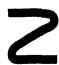
\includegraphics[keepaspectratio]{images/part001_73a6a0da.jpg}}

We recall that, by virtue of Ascoli's theorem (GT, X, §2, No.~5, Cor. 3 of Th. 2), a strictly compact subset H of \(\mathcal{K}(\mathrm{X};\mathrm{E})\) contained in \(\mathcal{K}(\mathrm{X},\mathrm{K};\mathrm{E})\) is characterized by the following conditions: \(1^{\circ}\) it is closed; \(2^{\circ}\) it is equicontinuous; \(3^{\circ}\) for every \(x\in \mathbf{K}\) , the set \(\mathrm{H}(x)\) is relatively compact in E.

COROLLARY. --- Let X be a paracompact, locally compact space; if E is a quasi-complete locally convex space, then the space \(\mathcal{K}(X;E)\) is quasi-complete.

It suffices, by virtue of Proposition 2, (ii), to note that for every compact subset K of X, \(\mathcal{K}(X,K;E)\) is a closed subspace of \(\mathcal{C}(K;E)\) , which is quasi-complete since every bounded subset of \(\mathcal{C}(K;E)\) consists of functions taking values in a same bounded subset of E.

\subsection{Approximation properties}

Lemma 1. --- Let X be a locally compact space, K a compact subset of X, and \((\mathrm{V}_{k})_{1\leqslant k\leqslant n}\) a finite covering of K by open sets of X. Then, there exist n continuous mappings \(f_{k}\) of X into {[}0,1{]}, such that the support of \(f_{k}\) is contained in \(V_{k}\) for \(1\leqslant k\leqslant n\) and such that \(\sum_{k=1}^{n}f_{k}(x)\leqslant1\) for all \(x\in X\) and \(\sum_{k=1}^{n}f_{k}(x)=1\) for all \(x\in K\) .

For, let \(X'\) be the compact space obtained by adjoining to X a point at infinity \(\omega\) (GT, I, §9, No.~8, Th. 4); the sets \(V_{0} = X' - K\) and \(V_{k}\) ( \(1 \leqslant k \leqslant n\) ) form an open covering of \(X'\) . Let \((f_{k})_{0 \leqslant k \leqslant n}\) be a continuous partition of unity subordinate to this covering of \(X'\) (GT, IX, §4, No.~3, Prop. 3); the functions \(f_{k}\) with index \(k \geqslant 1\) satisfy the conditions of the lemma.

Lemma 2. --- Let X be a locally compact space, K a compact subset of X, E a locally convex space, q a continuous semi-norm on E, and \(\Phi\) an equicontinuous set of mappings of X into E whose supports are contained in K. Then, for every \(\varepsilon > 0\) , there exists a continuous partition of unity \((\varphi_{j})_{0 \leqslant j \leqslant n}\) on X having the following properties:

\begin{enumerate}
\def\labelenumi{(\roman{enumi})}
\item
  \(\operatorname{Supp}(\varphi_j) \subset \mathrm{K}\) for \(1 \leqslant j \leqslant n\) .
\item
  If, for \(1 \leqslant j \leqslant n\) , \(x_j\) is any point of \(\operatorname{Supp}(\varphi_j)\) , then, for every function \(\mathbf{f} \in \Phi\) and every \(x \in \mathbf{X}\) ,
\end{enumerate}

\[
q \left(\mathbf {f} (x) - \sum_ {j = 1} ^ {n} \varphi_ {j} (x) \mathbf {f} \left(x _ {j}\right)\right) \leqslant \varepsilon .\tag{1}
\]

For every \(y\) belonging to the boundary of K, one has \(\mathbf{f}(y) = 0\) for all \(\mathbf{f} \in \Phi\) , therefore there exists an open neighborhood \(\mathrm{V}_y\) of \(y\) in X such that, for every \(z \in \mathrm{V}_y\) and every \(\mathbf{f} \in \Phi\) , one has \(q(\mathbf{f}(z)) \leqslant \varepsilon / 2\) . Let \(\mathrm{K}'\) be the set of points of K not belonging to any of the \(\mathrm{V}_y\) as \(y\) runs over the boundary of K; \(\mathrm{K}'\) is compact and is contained in the interior of K. The set \(\Phi\) is uniformly equicontinuous in K; therefore, there exists a finite open covering \((\mathrm{U}_j)_{1 \leqslant j \leqslant n}\) of \(\mathrm{K}'\) consisting of open sets in X contained in K, such that for every pair of points \(x, y\) of a same \(\mathrm{U}_j\) , one has \(q(\mathbf{f}(x) - \mathbf{f}(y)) \leqslant \varepsilon / 2\) for every \(\mathbf{f} \in \Phi\) . By Lemma 1, there exist \(n\) continuous mappings \(\varphi_j\) of X into {[}0,1{]} ( \(1 \leqslant j \leqslant n\) ) such that \(\operatorname{Supp}(\varphi_j) \subset \mathrm{U}_j\) and such that \(\sum_{j=1}^{n} \varphi_j(x) \leqslant 1\) on X and \(\sum_{j=1}^{n} \varphi_j(x) = 1\) on \(\mathrm{K}'\) . For \(x_j \in \operatorname{Supp}(\varphi_j)\) ( \(1 \leqslant j \leqslant n\) ) and \(\mathbf{f} \in \Phi\) , we therefore have, for all \(x \in \mathrm{U}_j\) ,

\[
q \big (\mathbf {f} (x) \varphi_ {j} (x) - \mathbf {f} (x _ {j}) \varphi_ {j} (x) \big) = \varphi_ {j} (x) q \big (\mathbf {f} (x) - \mathbf {f} (x _ {j}) \big) \leqslant \frac {\varepsilon}{2} \varphi_ {j} (x),
\]

and this relation remains true if \(x \notin U_{j}\) since then \(\varphi_{j}(x) = 0\) . By addition we infer that, for every \(x \in X\) ,

\[
q \left(\mathbf {f} (x) \left(1 - \varphi_ {0} (x)\right) - \sum_ {j = 1} ^ {n} \varphi_ {j} (x) \mathbf {f} \left(x _ {j}\right)\right) \leqslant \frac {\varepsilon}{2} \left(1 - \varphi_ {0} (x)\right),\tag{2}
\]

where \(\varphi_0 = 1 - \sum_{j=1}^{n} \varphi_j\) ; whence (1) for \(x \in \mathbf{K}'\) , since then \(\varphi_0(x) = 0\) ; (1) also holds for \(x \notin \mathbf{K}\) , the first member then being zero. Finally, for \(x \in \mathbf{K} - \mathbf{K}'\) we have \(q(\mathbf{f}(x)\varphi_0(x)) \leqslant \varepsilon/2\) by the definition of \(\mathbf{K}'\) , therefore this relation and (2) again imply (1) in this case.

Let X be a locally compact space; for every Banach space E (real or complex) we denote by \(\mathcal{C}^{b}(X;E)\) the vector space of continuous and bounded mappings of X into E; we know that the topology of uniform convergence in X is compatible with the vector space structure (real, resp. complex) of \(\mathcal{C}^{b}(X;E)\) , and it is defined by the norm

\[
\| \mathbf {f} \| = \sup _ {x \in X} \| \mathbf {f} (x) \|.\tag{3}
\]

Moreover, the normed space thus defined is a Banach space (GT, X, §3, No.~2, and No.~1, Cor. 2 of Prop. 2); the topology defined by this norm on \(\mathcal{K}(\mathrm{X};\mathrm{E})\) (in other words, the topology of uniform convergence in X) is coarser than the direct limit topology on \(\mathcal{K}(\mathrm{X};\mathrm{E})\) defined in No.~1.

PROPOSITION 3. --- Let X be a locally compact space, X' the compact space obtained by adjoining to X a point at infinity ω (GT, I, §9, No.~8,

Th. 4), and E a Banach space. The closure of \(\mathcal{K}(\mathrm{X};\mathrm{E})\) in the normed space \(\mathcal{C}^b (\mathrm{X};\mathrm{E})\) is the vector space of continuous functions on \(\mathbf{X}\) , with values in E and tending to 0 at the point \(\omega\) .

Let \(\mathbf{f} \in \mathcal{C}^b(\mathrm{X};\mathrm{E})\) be a function in the closure of \(\mathcal{K}(\mathrm{X};\mathrm{E})\) ; for every \(\varepsilon > 0\) , there exists a function \(\mathbf{g} \in \mathcal{K}(\mathrm{X};\mathrm{E})\) such that \(\| \mathbf{f}(x) - \mathbf{g}(x) \| \leqslant \varepsilon\) for all \(x \in \mathrm{X}\) ; if \(\mathrm{K}\) is the support of \(\mathbf{g}\) , it follows that \(\| \mathbf{f}(x) \| \leqslant \varepsilon\) for all \(x \in \complement \mathrm{K}\) , thus \(\mathbf{f}(x)\) tends to 0 as \(x\) tends to \(\omega\) . Conversely, if \(\mathbf{f}\) has this property then, for every \(\varepsilon > 0\) , there exists a compact set \(\mathrm{K} \subset \mathrm{X}\) such that \(\| \mathbf{f}(x) \| \leqslant \varepsilon\) for all \(x \in \complement \mathrm{K}\) . By Lemma 1 there exists a continuous mapping \(h\) of X into {[}0,1{]}, with compact support, equal to 1 on \(\mathrm{K}\) ; then \(\| \mathbf{f}(x) h(x) \| \leqslant \varepsilon\) on \(\complement \mathrm{K}\) and \(\mathbf{f}(x) = \mathbf{f}(x) h(x)\) on \(\mathrm{K}\) ; since \(\mathbf{f}h\) has compact support and \(\| \mathbf{f}(x) - \mathbf{f}(x) h(x) \| \leqslant 2\varepsilon\) for all \(x \in \mathrm{X}\) , the proposition is proved.

We shall denote by \(\mathcal{C}^{0}(\mathrm{X};\mathrm{E})\) the subspace of \(\mathcal{C}^{b}(\mathrm{X};\mathrm{E})\) formed by the functions tending to zero at the point at infinity \(\omega\) ; it is thus the completion of the normed space \(\mathcal{K}(\mathrm{X};\mathrm{E})\) .

PROPOSITION 4. --- Let X be a locally compact space, E a locally convex space; then, the space \(\mathcal{K}(\mathrm{X};\mathrm{E})\) is dense in \(\mathcal{C}(\mathrm{X};\mathrm{E})\) for the topology of compact convergence.

For every compact set \(K \subset X\) , there exists a function \(h \in \mathcal{K}(X; \mathbf{R})\) equal to 1 on K, by Lemma 1; for every function \(\mathbf{f} \in \mathcal{C}(X; E)\) the function hf, which belongs to \(\mathcal{K}(X; E)\) , is equal to f on K, whence our assertion.

PROPOSITION 5. --- Let X be a locally compact space, E a real (resp. complex) locally convex space. For every compact subset K of X, the vector space \(\mathcal{K}(X,K;\mathbf{R})\otimes_{\mathbf{R}}E\) (resp. \(\mathcal{K}(X,K;\mathbf{C})\otimes_{\mathbf{C}}E\) ) (identified with a set of mappings of X into E, cf.~A, II, §7, No.~7, Cor. of Prop. 15) is dense in \(\mathcal{K}(X,K;E)\) ; the vector space \(\mathcal{K}(X;\mathbf{R})\otimes_{\mathbf{R}}E\) (resp. \(\mathcal{K}(X;\mathbf{C})\otimes_{\mathbf{C}}E\) ) is dense in \(\mathcal{K}(X;E)\) .

As the second assertion is an obvious consequence of the first, it suffices to prove the latter. We apply Lemma 2 with \(\Phi\) reduced to a single element f of \(\mathcal{K}(X,K;E)\) ; then, for every \(x\in X\) ,

\[
q \left(f (x) - \sum_ {j = 1} ^ {n} \varphi_ {j} (x) f \left(x _ {j}\right)\right) \leqslant \varepsilon ,
\]

where the \(\varphi_{j}\) belong to \(\mathcal{K}(\mathrm{X},\mathrm{K};\mathbf{R})\) ; since the mapping \(x\mapsto \sum_{j = 1}^{n}\varphi_{j}(x)f(x_{j})\) may be canonically identified with the element \(\sum_{j = 1}^{n}\varphi_{j}\otimes f(x_{j})\) , this proves the proposition, by the definition of the topology of \(\mathcal{K}(\mathrm{X},\mathrm{K};\mathrm{E})\) .

\subsection{Definition of a measure}

DEFINITION 2. --- A continuous linear form on \(\mathcal{K}(\mathrm{X};\mathbf{C})\) , \(\mathrm{X}\) a locally compact space, is called a measure (or complex measure) on \(\mathrm{X}\) .

If \(\mu\) is a measure on a locally compact space \(X\) , the value of the measure for a function \(f \in \mathcal{K}(X; \mathbf{C})\) is called the integral of \(f\) with respect to \(\mu\) ; besides the general notations \(\mu(f)\) and \(\langle f, \mu \rangle\) , one also uses the notations \(\int f d\mu, \int f\mu, \int f(x) d\mu(x)\) and \(\int f(x)\mu(x)\) to denote it; as to the use of the letter \(x\) , see S, I, §1, No.~1.

By virtue of the criterion for continuity in direct limits (TVS, Ch. II, §4, No.~4, Prop. 5), to say that \(\mu\) is a measure on X means that \(\mu\) is a linear form on \(\mathcal{K}(\mathrm{X};\mathbf{C})\) satisfying the following condition: for every compact subset K of X, there exists a number \(\mathrm{M_K}\) such that, for every function \(f\in \mathcal{K}(\mathrm{X};\mathbf{C})\) whose support is contained in K,

\[
| \mu (f) | \leqslant \mathrm{M} _ {\mathrm{K}} \cdot \| f \| \quad (\text { where } \| f \| = \sup _ {x \in \mathrm{X}} | f (x) |).\tag{4}
\]

More generally:

PROPOSITION 6. --- Let X be a locally compact space, \((\mathrm{K}_{\alpha})\) a family of compact subsets of X whose interiors \(\mathring{K}_{\alpha}\) form an open covering of X. For a linear form \(\mu\) on \(\mathcal{K}(\mathrm{X};\mathbf{C})\) to be a measure on X, it is necessary and sufficient that, for every \(\alpha\) , there exist a number \(M_{\alpha}\) such that

\[
| \mu (f) | \leqslant \mathrm{M} _ {\alpha} \cdot \| f \|\tag{5}
\]

for every function \(f \in \mathcal{K}(\mathrm{X}, \mathrm{K}_{\alpha}; \mathbf{C})\) .

The condition being obviously necessary, it suffices to prove that (5) implies (4) for every compact subset K of X. Now, K is covered by a finite number of open sets \(\mathring{K}_{\alpha_{i}}\) ( \(1 \leqslant i \leqslant n\) ); applying Lemma 1 of No.~2 to K and to the \(\mathring{K}_{\alpha_{i}}\) , there exist continuous functions \(g_{i} \geqslant 0\) on X such that \(\operatorname{Supp}(g_{i}) \subset \mathrm{K}_{\alpha_{i}}\) , \(0 \leqslant \sum_{i=1}^{n} g_{i}(x) \leqslant 1\) for all \(x \in X\) and \(\sum_{i=1}^{n} g_{i}(x) = 1\) for \(x \in K\) . For every function \(f \in \mathcal{K}(X, K; \mathbf{C})\) , we can therefore write \(f = \sum_{i=1}^{n} fg_{i}\) and we have \(fg_{i} \in \mathcal{K}(X, K_{\alpha_{i}}; \mathbf{C})\) and \(\|fg_{i}\| \leqslant \|f\|\) ; if \(M_{K} = \sum_{i=1}^{n} M_{\alpha_{i}}\) , we then have the relation (4).

We denote by \(\mathcal{M}(\mathrm{X};\mathbf{C})\) , or simply \(\mathcal{M}(\mathrm{X})\) if no confusion can result, the vector space of measures on \(\mathrm{X}\) , in other words, the dual of \(\mathcal{K}(\mathrm{X};\mathbf{C})\) .

One knows that for every set \(\mathfrak{S}\) of bounded subsets of \(\mathcal{K}(\mathrm{X};\mathbf{C})\) , there is defined on \(\mathcal{M}(\mathrm{X};\mathbf{C})\) the \(\mathfrak{S}\) -topology, which is locally convex (TVS, III, §3, No.~1, Cor. of Prop. 1). We denote the topological vector space, obtained by equipping \(\mathcal{M}(\mathrm{X};\mathbf{C})\) with the \(\mathfrak{S}\) -topology, by \(\mathcal{M}_{\mathfrak{S}}(\mathrm{X};\mathbf{C})\) or \(\mathcal{M}_{\mathfrak{S}}(\mathrm{X})\) .

PROPOSITION 7. --- For every set S of bounded subsets of \(\mathcal{K}(\mathrm{X};\mathbf{C})\) that is a covering of \(\mathcal{K}(\mathrm{X};\mathbf{C})\) , the space \(\mathcal{M}_{\mathfrak{S}}(\mathrm{X};\mathbf{C})\) is Hausdorff and quasi-complete.

This results from the fact that \(\mathcal{K}(\mathrm{X};\mathbf{C})\) is barreled (TVS, III, §4, No.~2, Cor. 4 of Th. 1).

Examples of measures. --- I. Atomic measures. Let X be a locally compact space, a a point of X; the mapping \(f \mapsto f(a)\) of \(\mathcal{K}(\mathrm{X};\mathbf{C})\) into C obviously satisfies the condition (4) with \(M_{K} = 1\) for every compact subset K of X containing a, hence is a measure on X, which is denoted by \(\varepsilon_{a}\) ; it is called the Dirac measure at the point a, or the measure defined by a unit mass placed at the point a.

More generally, let \(\alpha\) be a mapping of X into C such that, for every compact subset K of X, \(\sum_{x\in K}|\alpha(x)|<+\infty\) . Then, for every function \(f\in\mathcal{K}(X,K;\mathbf{C})\) , the sum

\[
\mu (f) = \sum_ {x \in X} \alpha (x) f (x)
\]

is defined, being equal to \(\sum_{x\in K}\alpha (x)f(x)\) ; it is clear that \(\mu\) is a linear form on \(\mathcal{K}(\mathrm{X};\mathbf{C})\) and that, for \(f\in \mathcal{K}(\mathrm{X},\mathrm{K};\mathbf{C})\) ,

\[
| \mu (f) | \leqslant \left(\sum_ {x \in K} | \alpha (x) |\right) \cdot \| f \|,
\]

in other words the condition (4) is satisfied.

A measure \(\mu\) on X is said to be atomic if there exists a mapping \(\alpha\) of X into C such that \(\sum_{x\in K}|\alpha (x)| < +\infty\) for every compact subset K of X, and such that \(\mu\) is equal to the measure defined as above. If N is the set of \(x\in X\) such that \(\alpha (x)\neq 0\) , the condition imposed on \(\alpha\) implies that for every compact subset K of X, \(\mathrm{K}\cap \mathrm{N}\) is countable. One also says that \(\mu\) is defined by the masses \(\alpha (x)\) placed at the points \(x\in \mathrm{N}\) . If one assumes that \(\mathrm{N}\cap \mathrm{K}\) is finite for every compact set \(\mathrm{K}\subset \mathrm{X}\) , then obviously \(\sum_{x\in K}|\alpha (x)| < +\infty\) ; it comes to the same to say that N is a closed and discrete subspace of X, because then every point of X has a compact neighborhood containing only a finite number of points of N, and conversely, if this is the case, then every compact subset of X can be covered by a finite number of such neighborhoods. When N is closed and discrete, every atomic measure defined by a function \(\alpha\) such that \(\alpha(x)=0\) on CN is called a discrete measure on X (cf.~§2, No.~5).

\begin{enumerate}
\def\labelenumi{\Roman{enumi}.}
\setcounter{enumi}{1}
\tightlist
\item
  Lebesgue measure. For every function \(f \in \mathcal{K}(\mathbf{R}; \mathbf{C})\) , there exists a compact interval \([a, b]\) of R outside of which f is zero. The integral
\end{enumerate}

\[
\operatorname{I} (f) = \int_ {- \infty} ^ {+ \infty} f (x) d x = \int_ {a} ^ {b} f (x) d x
\]

is therefore defined; moreover, by the theorem of the mean (FRV, II, §1, No.~5, Prop. 6), we have \(|\mathrm{I}(f)| \leqslant (b - a) \| f \|\) ; this shows that \(f \mapsto \mathrm{I}(f)\) is a measure on \(\mathbf{R}\) , which is called Lebesgue measure.

For every interval J (bounded or not) of R, one similarly calls Lebesgue measure on J the measure \(f \mapsto \int_{J} f(x) dx\) , a linear form on \(\mathcal{K}(J; \mathbf{C})\) (the integral having meaning since there exists a compact interval \([a, b]\) contained in J outside of which f is zero).

\begin{enumerate}
\def\labelenumi{\Roman{enumi}.}
\setcounter{enumi}{2}
\tightlist
\item
  Let g be a continuous mapping of a compact interval \(I \subset R\) into C, having a continuous derivative in I. Let \(\Gamma = g(I)\) , which is a compact subspace of C; the mapping
\end{enumerate}

\[
f \mapsto \int_ {\mathrm{I}} f (g (t)) g ^ {\prime} (t) d t
\]

of \(\mathcal{C}(\Gamma;\mathbf{C})\) into C is a continuous linear form by virtue of the theorem of the mean, hence is a complex measure on \(\Gamma\) ; the integral relative to this measure is also written \(\int_{\Gamma} f(z) dz\) , even though it depends not only on \(\Gamma\) but also on g.

Remark. --- The giving of a measure \(\mu\) on a locally compact space X defines on X (along with the topology of X) a structure S. Let \(X_{1}\) be a second set, \(\varphi\) a bijective mapping of X onto \(X_{1}\) ; in conformity with general definitions (S, R, §8), the structure \(S_{1}\) obtained by transporting to \(X_{1}\) the structure S of X, by means of \(\varphi\) , is defined in the following way. The topology of X is transported to \(X_{1}\) by \(\varphi\) ; the functions of \(\mathcal{K}(X_{1};\mathbf{C})\) are then the functions f such that \(f \circ \varphi\) belongs to \(\mathcal{K}(X;\mathbf{C})\) , and the measure \(\mu_{1}\) on \(X_{1}\) is defined by \(\mu_{1}(f) = \mu(f \circ \varphi)\) .

In particular, an automorphism of the structure S is a homeomorphism \(\sigma\) of X onto itself, such that

\[
\mu (f) = \mu (f \circ \sigma)
\]

for every function \(f \in \mathcal{K}(\mathrm{X};\mathbf{C})\) ; the measure \(\mu\) is then also said to be invariant under the homeomorphism \(\sigma\) .

Example. --- Lebesgue measure on \(\mathbf{R}\) is invariant under every translation of the additive group \(\mathbf{R}\) . Indeed, for every function \(f \in \mathcal{K}(\mathbf{R}; \mathbf{C})\) and every real number \(a\) , we have

\[
\int_ {- \infty} ^ {+ \infty} f (x + a) d x = \int_ {- \infty} ^ {+ \infty} f (t) d t
\]

by the change-of-variables formula (FRV, II, §2, No.~1, formula (1)).

For a generalization, see Ch. VII, §1, No.~2, Th. 1.

\subsection{Product of a measure by a continuous function}

Let X be a locally compact space, g a continuous mapping of X into C. It is clear that \(f \mapsto gf\) is a linear mapping of \(\mathcal{K}(\mathrm{X};\mathbf{C})\) into itself; let us show that this mapping is continuous. Indeed, for every compact subset K of X, and for every function \(f \in \mathcal{K}(\mathrm{X},\mathrm{K};\mathbf{C})\) , we have \(gf \in \mathcal{K}(\mathrm{X},\mathrm{K};\mathbf{C})\) ; moreover, if \(b_{\mathrm{K}} = \sup_{x \in \mathrm{K}} |g(x)|\) then \(\|gf\| \leqslant b_{\mathrm{K}} \|f\|\) , whence our assertion (TVS, II, §4, No.~4, Prop. 5). The transpose of this continuous linear mapping (TVS, II, §6, No.~4) is therefore a linear mapping of \(\mathcal{M}(\mathrm{X};\mathbf{C})\) into itself, which is denoted \(\mu \mapsto g \cdot \mu\) (or \(\mu \mapsto g\mu\) , if no confusion can result). If \(\nu = g \cdot \mu\) we therefore have, for every function \(f \in \mathcal{K}(\mathrm{X};\mathbf{C})\) ,

\[
\langle f, \nu \rangle = \langle g f, \mu \rangle\tag{6}
\]

or again

\[
\int f (x) d \nu (x) = \int f (x) g (x) d \mu (x)
\]

(which is abbreviated in the form \(d\nu(x) = g(x) \, d\mu(x)\) ). One says that \(g \cdot \mu\) is the product of the measure \(\mu\) by the function \(g\) , or also the measure with density \(g\) with respect to \(\mu\) (cf.~Ch. V, §5, No.~2, Def. 2). If \(g_1, g_2\) are two continuous mappings of X into C, and \(\mu_1, \mu_2\) are two measures on X, then

\[
\begin{array}{c} (g _ {1} + g _ {2}) \cdot \mu = g _ {1} \cdot \mu + g _ {2} \cdot \mu , \quad g \cdot (\mu_ {1} + \mu_ {2}) = g \cdot \mu_ {1} + g \cdot \mu_ {2}, \\ (g _ {1} g _ {2}) \cdot \mu = g _ {1} \cdot (g _ {2} \cdot \mu). \end{array}
\]

Moreover, \(1 \cdot \mu = \mu\) (here 1 denotes the constant function equal to 1 on X); the set \(\mathcal{M}(\mathrm{X};\mathbf{C})\) , equipped with the external law of composition \((g,\mu) \mapsto g \cdot \mu\) and with its additive structure, is thus a module over the ring \(\mathcal{C}(\mathrm{X};\mathbf{C})\) .

\subsection{Real measures. Positive measures}

Let X be a locally compact space. The real vector space \(\mathcal{K}(\mathrm{X};\mathbf{R})\) is a subspace of the real vector space underlying the complex vector space \(\mathcal{K}(\mathrm{X};\mathbf{C})\) ; moreover, the mapping \((f_{1},f_{2})\mapsto f_{1}+if_{2}\) is an isomorphism of the product topological vector space \(\mathcal{K}(\mathrm{X};\mathbf{R})\times\mathcal{K}(\mathrm{X};\mathbf{R})\) onto the real topological vector space \(\mathcal{K}(\mathrm{X};\mathbf{C})\) (No.~1, Prop. 1).

For every (complex) measure \(\mu\in\mathcal{M}(\mathrm{X};\mathbf{C})\) , the restriction \(\mu_{0}\) of \(\mu\) to \(\mathcal{K}(\mathrm{X};\mathbf{R})\) is a continuous R-linear mapping of \(\mathcal{K}(\mathrm{X};\mathbf{R})\) into C; moreover, this restriction determines \(\mu\) , since if \(f=f_{1}+if_{2}\) with \(f_{1},f_{2}\) in \(\mathcal{K}(\mathrm{X};\mathbf{R})\) , then \(\mu(f)=\mu_{0}(f_{1})+i\mu_{0}(f_{2})\) . Conversely, let \(\mu_{0}\) be a continuous R-linear mapping of \(\mathcal{K}(\mathrm{X};\mathbf{R})\) into C; it is clear that the mapping

\[
f _ {1} + i f _ {2} \mapsto \mu_ {0} (f _ {1}) + i \mu_ {0} (f _ {2})
\]

is a (complex) measure on X. Thus, every measure on X may be identified with its restriction to \(\mathcal{K}(\mathrm{X};\mathbf{R})\) .

Let \(\mu\) be a measure on X. One calls conjugate measure of \(\mu\) the measure \(\overline{\mu}\) defined by \(\overline{\mu}(f) = \overline{\mu(\overline{f})}\) for every function \(f \in \mathcal{K}(\mathrm{X};\mathbf{C})\) ; for, it is clear that \(\overline{\mu}\) is a C-linear form and that it is continuous on \(\mathcal{K}(\mathrm{X};\mathbf{C})\) ; obviously \(\overline{\overline{\mu}} = \mu\) , and, for two measures \(\mu, \nu\) and two scalars \(\alpha, \beta\) in \(\mathbf{C}\) ,

\[
\overline {{(\alpha \mu + \beta \nu)}} = \overline {{\alpha}} \cdot \overline {{\mu}} + \overline {{\beta}} \cdot \overline {{\nu}}.
\]

More generally, for every function \(g \in \mathcal{C}(\mathrm{X};\mathbf{C})\) and every measure \(\mu\) on \(\mathbf{X}\) ,

\[
\overline {{{g \cdot \mu}}} = \overline {{{g}}} \cdot \overline {{{\mu}}},\tag{7}
\]

as is immediate from the definition (No.~4).

A measure \(\mu\) on X is said to be real if \(\overline{\mu} = \mu\) ; by the foregoing, it is the same to say that for every function \(f \in \mathcal{K}(X; \mathbf{R})\) , \(\mu(f)\) is a real number. If one identifies a real measure with its restriction to \(\mathcal{K}(X; \mathbf{R})\) , one can thus say that the set of real measures on X is the dual of the real locally convex space \(\mathcal{K}(X; \mathbf{R})\) ; it is a real vector space that is denoted \(\mathcal{M}(X; \mathbf{R})\) (or sometimes \(\mathcal{M}(X)\) if this does not cause any confusion). The Lebesgue measure on R is a real measure, as is the Dirac measure \(\varepsilon_{a}\) for every point \(a \in X\) . If \(g \in \mathcal{C}(X; \mathbf{R})\) and if \(\mu\) is a real measure, then so is \(g \cdot \mu\) by virtue of (7).

Let \(\mu\) be a (complex) measure on X. It follows from the preceding definition that the measures \(\mu_{1} = (\mu +\overline{\mu}) / 2\) and \(\mu_{2} = (\mu -\overline{\mu}) / 2i\) are real; they are called, respectively, the real part and the imaginary part of \(\mu\) , and they are denoted by \(\mathcal{R}\mu\) and \(\mathcal{I}\mu\) , respectively; these measures are also characterized by the fact that, for every function \(f\in \mathcal{K}(\mathbf{X};\mathbf{R})\) ,

\[
\mu_ {1} (f) = \mathcal {R} (\mu (f)), \quad \mu_ {2} (f) = \mathcal {I} (\mu (f)).
\]

Obviously

\[
\mu = \mu_ {1} + i \mu_ {2}, \quad \overline {{{{\mu}}}} = \mu_ {1} - i \mu_ {2}.
\]

The space \(\mathcal{K}(\mathrm{X};\mathbf{R})\) of continuous real-valued functions on \(\mathrm{X}\) with compact support is clearly a Riesz space for the order relation \(f\leqslant g\) . We shall say that a real measure \(\mu\) on \(\mathrm{X}\) is positive if \(\mu (f)\geqslant 0\) for every function \(f\geqslant 0\) belonging to \(\mathcal{K}(\mathrm{X};\mathbf{R})\) ; it is thus a positive linear form on the Riesz space \(\mathcal{K}(\mathrm{X};\mathbf{R})\) (Ch. II, §2, No.~1, Def. 1). Conversely:

THEOREM 1. --- Every positive linear form on the Riesz space \(\mathcal{K}(\mathrm{X};\mathbf{R})\) is a (positive) real measure on \(\mathrm{X}\) .

For, let \(\mu\) be a positive linear form on \(\mathcal{K}(\mathrm{X};\mathbf{R})\) and let \(\mathrm{K}\) be a compact subset of \(\mathrm{X}\) . There exists a continuous mapping \(f_0\) of \(\mathrm{X}\) into {[}0, 1{]}, with compact support, such that \(f_0(x) = 1\) on \(\mathrm{K}\) (No.~2, Lemma 1). For every function \(g \in \mathcal{K}(\mathrm{X},\mathrm{K};\mathbf{R})\) , we thus have \(-\| g \| f_0 \leqslant g \leqslant \| g \| f_0\) , consequently \(|\mu(g)| \leqslant \| g \| \cdot \mu(f_0)\) , which proves the theorem.

We denote by \(\mathcal{M}_{+}(X)\) the pointed convex cone of positive measures on X (or, what amounts to the same thing, the cone of positive linear forms on the Riesz space \(\mathcal{K}(X;\mathbf{R})\) ).

THEOREM 2. --- Every real measure on a locally compact space X is the difference of two positive measures.

In view of Theorem 1 and Ch. II, §2, No.~2, Th. 1, it all comes down to proving that a real measure \(\mu\) on X is a relatively bounded linear form on the Riesz space \(\mathcal{K}(\mathrm{X};\mathbf{R})\) . Let \(f\) be a continuous function \(\geqslant 0\) on X, with compact support K; the relation \(0 \leqslant g \leqslant f\) in \(\mathcal{K}(\mathrm{X};\mathbf{R})\) implies that \(\|g\| \leqslant \|f\|\) and that the support of \(g\) is contained in K. By hypothesis, there exists a number \(\mathrm{M}_{\mathrm{K}} \geqslant 0\) such that \(|\mu(h)| \leqslant \mathrm{M}_{\mathrm{K}} \cdot \|h\|\) for every function \(h \in \mathcal{K}(\mathrm{X},\mathrm{K};\mathbf{R})\) ; therefore \(|\mu(g)| \leqslant \mathrm{M}_{\mathrm{K}} \cdot \|g\| \leqslant \mathrm{M}_{\mathrm{K}} \cdot \|f\|\) , which proves the theorem.

The space \(\mathcal{M}(\mathrm{X};\mathbf{R})\) of real measures on X is thus identical with the space of relatively bounded linear forms on the Riesz space \(\mathcal{K}(\mathrm{X};\mathbf{R})\) ; we recall that in \(\mathcal{M}(\mathrm{X};\mathbf{R})\) , the order relation \(\mu\leqslant\nu\) signifies that \(\nu-\mu\) is a positive measure, or also that \(\mu(f)\leqslant\nu(f)\) for every function \(f\in\mathcal{K}_{+}(\mathrm{X})\) .

THEOREM 3. --- The space \(\mathcal{M}(\mathrm{X};\mathbf{R})\) of real measures on a locally compact space X is fully lattice-ordered.

This follows from Ch. II, §2, No.~2, Th. 1.

In conformity with the notations of Ch. II, §1, we define, for every real measure \(\mu\) on \(X\) ,

\[
\mu^ {+} = \sup (\mu , 0), \quad \mu^ {-} = \sup (- \mu , 0), \quad | \mu | = \sup (\mu , - \mu);
\]

then \(\mu = \mu^{+} - \mu^{-}\) , \(|\mu| = \mu^{+} + \mu^{-}\) and \(\inf (\mu^{+},\mu^{-}) = 0\) . Moreover, for every function \(f\in \mathcal{K}_{+}(\mathrm{X})\) ,

\[
\int f d \mu^ {+} = \sup _ {0 \leqslant g \leqslant f, g \in \mathcal {K} (\mathrm{X})} \int g d \mu\tag{8}
\]

and

\[
\int f d | \mu | = \sup _ {| g | \leqslant f, g \in \mathcal {K} (\mathrm{X})} \int g d \mu ,\tag{9}
\]

whence, in particular,

\[
\left| \int f d \mu \right| \leqslant \int | f | d | \mu |\tag{10}
\]

for every function \(f \in \mathcal{K}(\mathbf{X};\mathbf{R})\) .

This inequality is also true if \(f \in \mathcal{K}(\mathrm{X};\mathbf{C})\) ; for, on multiplying f by a complex number of absolute value 1 (which does not change either side of the inequality), one can suppose that \(\int f d\mu \geqslant 0\) . Then

\[
\left| \int f d \mu \right| = \int f d \mu = \int (\mathcal {R} f) d \mu \leqslant \int | \mathcal {R} f | d | \mu | \leqslant \int | f | d | \mu |.
\]

\subsection{Absolute value of a complex measure}

Let \(\mu\) be a complex measure on a locally compact space \(X\) ; for every function \(f \in \mathcal{K}_{+}(X)\) , the positive real number

\[
L (f) = \sup _ {| g | \leqslant f, g \in \mathcal {K} (\mathrm{X}; \mathbf {C})} \left| \int g d \mu \right|\tag{11}
\]

is finite, because the relation \(|g| \leqslant f\) implies that \(\operatorname{Supp}(g) \subset \operatorname{Supp}(f)\) and \(\| g \| \leqslant \| f \|\) , thus our assertion follows from formula (4) of No.~3. Let us show that \(L\) can be extended, in only one way, to a positive measure on \(X\) ; in view of No.~5, Th. 1 and Ch. II, §2, No.~1, Prop. 3, it will suffice to show that if \(f_1, f_2\) are two functions in \(\mathcal{K}_+(X)\) , then \(L(f_1 + f_2) = L(f_1) + L(f_2)\) . Now, if \(|g_1| \leqslant f_1\) and \(|g_2| \leqslant f_2\) , where \(g_1\) and \(g_2\) are functions in \(\mathcal{K}(X; \mathbf{C})\) , we have \(|g_1 + \zeta g_2| \leqslant f_1 + f_2\) for any complex number \(\zeta\) of absolute value 1, therefore

\[
\left| \mu (g _ {1} + \zeta g _ {2}) \right| = \left| \mu (g _ {1}) + \zeta \mu (g _ {2}) \right| \leqslant L (f _ {1} + f _ {2}).
\]

Moreover, we can suppose \(\zeta\) so chosen that

\[
\left| \mu (g _ {1}) + \zeta \mu (g _ {2}) \right| = \left| \mu (g _ {1}) \right| + \left| \mu (g _ {2}) \right|;
\]

since \(|\mu(g_i)|\) is arbitrarily close to \(L(f_i)\) ( \(i = 1,2\) ), this proves that \(L(f_1) + L(f_2) \leqslant L(f_1 + f_2)\) . On the other hand, consider a function \(g \in \mathcal{K}(\mathbf{X};\mathbf{C})\) such that \(|g| \leqslant f_1 + f_2\) . The function \(g_i\) equal to \(g f_i / (f_1 + f_2)\) at the points where \(f_1(x) + f_2(x) \neq 0\) , and to 0 elsewhere ( \(i = 1,2\) ), is continuous on \(\mathbf{X}\) because \(f_i / (f_1 + f_2)\) ( \(i = 1,2\) ) is continuous at every point where \(f_1(x) + f_2(x) \neq 0\) and we have \(|g_i(x)| \leqslant |g(x)|\) for every \(x \in \mathbf{X}\) , which proves the continuity of \(g_i\) at the points where \(f_1(x) + f_2(x) = 0\) ( \(i = 1,2\) ), since at these points we have also \(g(x) = 0\) . It is clear that \(|g_i| \leqslant f_i\) ( \(i = 1,2\) ) and \(g = g_1 + g_2\) , therefore

\[
| \mu (g) | \leqslant | \mu (g _ {1}) | + | \mu (g _ {2}) | \leqslant L (f _ {1}) + L (f _ {2});
\]

since \(|\mu(g)|\) is arbitrarily close to \(L(f_1 + f_2)\) , we have

\[
L (f _ {1} + f _ {2}) \leqslant L (f _ {1}) + L (f _ {2}),
\]

which completes the proof of our assertion.

When \(\mu\) is a real measure, it follows from formula (9) that \(|\mu| \leqslant L\) ; on the other hand, by virtue of the last part of No.~5, if \(g \in \mathcal{K}(\mathbf{X}; \mathbf{C})\) and \(|g| \leqslant f \in \mathcal{K}_{+}(\mathbf{X})\) then \(|\int g d\mu| \leqslant \int |g| \cdot d|\mu| \leqslant \int f d|\mu|\) , therefore by definition \(L \leqslant |\mu|\) , in other words \(L = |\mu|\) .

We denote again by \(|\mu|\) the positive measure L for any complex measure \(\mu\) , and we say that \(|\mu|\) is the absolute value of \(\mu\) . The definition of \(|\mu|\) can therefore be written

\[
| \mu | (f) = \sup _ {| g | \leqslant f, g \in \mathcal{K} (\mathrm{X}; \mathbf {C})} | \mu (g) |,\tag{12}
\]

consequently, for every function \(g \in \mathcal{K}(\mathrm{X};\mathbf{C})\)

\[
\left| \int g d \mu \right| \leqslant \int | g | d | \mu |.\tag{13}
\]

It is clear that for every scalar \(\alpha \in \mathbf{C}\) and every measure \(\mu\) on \(X\) ,

\[
| \alpha \mu | = | \alpha | \cdot | \mu |.\tag{14}
\]

On the other hand, if \(\mu\) and \(\nu\) are two measures on \(X\) , \(f\) is a function in \(\mathcal{K}_{+}(X)\) , and \(g\) is a function in \(\mathcal{K}(X; \mathbf{C})\) such that \(|g| \leqslant f\) , then

\[
\left| \int g d (\mu + \nu) \right| = \left| \int g d \mu + \int g d \nu \right| \leqslant \int f d | \mu | + \int f d | \nu |,
\]

whence

\[
| \mu + \nu | \leqslant | \mu | + | \nu |.\tag{15}
\]

With the same notations, the relations \(|g| \leqslant f\) and \(|\overline{g}| \leqslant f\) are equivalent, therefore

\[
| \overline {{{\mu}}} | = | \mu |.\tag{16}
\]

It follows from (14), (15) and (16) that

\[
| \mathcal {R} \mu | \leqslant | \mu |, \quad | \mathcal {I} \mu | \leqslant | \mu |, \quad | \mu | \leqslant | \mathcal {R} \mu | + | \mathcal {I} \mu |.\tag{17}
\]

PROPOSITION 8. --- If \(\mu\) is a measure on X then, for every function \(h \in \mathcal{C}(\mathrm{X};\mathbf{C})\) ,

\[
\left| h \cdot \mu \right| \leqslant \left| h \right| \cdot \left| \mu \right|.\tag{18}
\]

For, if \(f \in \mathcal{K}_+(\mathbf{X})\) and if \(g \in \mathcal{K}(\mathbf{X};\mathbf{C})\) is such that \(|g| \leqslant f\) , then, by (13), \(|\int gh d\mu| \leqslant \int |gh| d|\mu| \leqslant \int f|h| d|\mu|\) , which proves (18).

\subsection{Definition of a measure by extension}

Let X be a locally compact space; if V is a dense linear subspace of \(\mathcal{K}(\mathrm{X};\mathbf{C})\) , it is clear that two measures \(\mu_{1}, \mu_{2}\) on X that coincide on V are equal, and that every linear form on V that is continuous for the topology induced by that of \(\mathcal{K}(\mathrm{X};\mathbf{C})\) may be extended (in only one way) to a measure on X. For positive measures, a convenient criterion is the following:

PROPOSITION 9. --- Let V be a linear subspace of \(\mathcal{K}(\mathbf{X};\mathbf{R})\) having the following property:

\begin{enumerate}
\def\labelenumi{(\Alph{enumi})}
\setcounter{enumi}{15}
\tightlist
\item
  For every compact subset \(\mathbf{K}\) of \(\mathbf{X}\) , there exists a function \(f \in \mathbf{V}\) such that \(f \geqslant 0\) and such that \(f(x) > 0\) for all \(x \in \mathbf{K}\) .
\end{enumerate}

Under these conditions, every positive linear form on V for the ordering induced by that of \(\mathcal{K}(\mathrm{X};\mathbf{R})\) (Ch. II, §2, No.~1, Def. 1) may be extended to a positive measure on X (which is unique when V is dense in \(\mathcal{K}(\mathrm{X};\mathbf{R})\) ).

For every function \(f \in \mathcal{K}(\mathbf{X};\mathbf{R})\) , with support \(K\) , there exists a function \(g \in V\) such that \(f \leqslant g\) ; for, there exists a function \(h \geqslant 0\) in \(V\) such that \(h(x) > 0\) for all \(x \in K\) ; setting \(\alpha = \inf_{x \in K} h(x)\) , we thus have \(\alpha > 0\) and the function \(g = (\alpha^{-1} \|f\|)h\) meets the requirements. It then suffices to apply Th. 1 of No.~5 and Prop. 1 of TVS, II, §3, No.~1.

\subsection{Bounded measures}

Let X be a locally compact space. Since the topology on \(\mathcal{K}(X;\mathbf{C})\) induced by that of \(\mathcal{C}^{b}(X;\mathbf{C})\) is coarser than the direct limit topology on \(\mathcal{K}(X;\mathbf{C})\) , a measure on X is not necessarily continuous for the topology of uniform convergence in X.

DEFINITION 3. --- A measure on a locally compact space X is said to be bounded if it is continuous on \(\mathcal{K}(\mathrm{X};\mathbf{C})\) for the topology of uniform convergence.

It comes to the same to say that there exists a finite number \(M \geqslant 0\) such that, for every function \(f \in \mathcal{K}(\mathbf{X}; \mathbf{C})\) ,

\[
| \mu (f) | \leqslant \mathrm{M} \| f \|\tag{19}
\]

(where \(\| f\|\) is defined by formula (3) of No.~2).

To say that \(\mu\) is a bounded measure thus signifies that \(\mu\) belongs to the dual of the space \(\mathcal{K}(\mathrm{X};\mathbf{C})\) normed by \(\| f\|\) ; we shall denote this dual by \(\mathcal{M}^1 (\mathrm{X};\mathbf{C})\) (or simply \(\mathcal{M}^1 (\mathrm{X})\) when no confusion can result). We know that \(\mathcal{M}^1 (\mathrm{X};\mathbf{C})\) is equipped with a norm, \(\| \mu \|\) being the smallest of the numbers \(M\geqslant 0\) for which the inequality (19) holds for every function \(f\in \mathcal{K}(\mathrm{X};\mathbf{C})\) , or again,

\[
\| \mu \| = \sup _ {\| f \| \leqslant 1, f \in \mathcal{K} (\mathrm{X}; \mathbf {C})} | \mu (f) |.\tag{20}
\]

Equipped with this norm, \(\mathcal{M}^{1}(X;\mathbf{C})\) is known to be a Banach space (TVS, III, §3, No.~8, Cor. 2 of Prop. 12).

The definition of \(\|\mu\|\) by the formula (20) may be extended to every measure \(\mu\) on X and, by an abuse of language, \(\|\mu\|\) is again said to be the norm of \(\mu\) ; for \(\mu\) to be bounded, it is necessary and sufficient that \(\|\mu\|\) be finite.

If X is compact, then every measure on X is bounded.

Examples. --- 1) The measure \(\varepsilon_{a}\) defined by a unit mass at a point \(a \in X\) is bounded, and \(\| \varepsilon_{a} \| = 1\) .

\begin{enumerate}
\def\labelenumi{\arabic{enumi})}
\setcounter{enumi}{1}
\tightlist
\item
  The Lebesgue measure on \(\mathbf{R}\) is not bounded; indeed, for every integer \(n > 0\) there exists a function \(f \in \mathcal{K}(\mathbf{R}; \mathbf{C})\) with values in {[}0,1{]} and equal to 1 on the interval \([-n, n]\) (No.~2, Lemma 1); thus \(\| f \| = 1\) and
\end{enumerate}

\[
\int_ {- \infty} ^ {+ \infty} f (x) d x \geqslant \int_ {- n} ^ {n} f (x) d x = 2 n,
\]

which proves that there does not exist any finite number \(M\) satisfying the relation (19).

\begin{enumerate}
\def\labelenumi{\arabic{enumi})}
\setcounter{enumi}{2}
\tightlist
\item
  On the real line \(\mathbf{R}\) , the mapping
\end{enumerate}

\[
f \mapsto \int_ {- \infty} ^ {+ \infty} \frac {f (x) d x}{1 + x ^ {2}}
\]

is a bounded measure since, for every function \(f \in \mathcal{K}(\mathbf{R};\mathbf{C})\) ,

\[
\left| \int_ {- \infty} ^ {+ \infty} \frac {f (x) d x}{1 + x ^ {2}} \right| \leqslant \| f \| \int_ {- \infty} ^ {+ \infty} \frac {d x}{1 + x ^ {2}} = \pi \cdot \| f \|.
\]

Since the relations \(\| f\| \leqslant 1\) and \(\| \overline{f}\| \leqslant 1\) are equivalent, it follows from (20) that

\[
\| \overline {{\mu}} \| = \| \mu \|\tag{21}
\]

for every measure \(\mu\) on X.

PROPOSITION 10. --- For every measure \(\mu\) on X,

\[
\| \mu \| = \sup _ {0 \leqslant f \leqslant 1, f \in \mathcal {K} (\mathrm{X}; \mathbf {R})} | \mu | (f).\tag{22}
\]

For, taking into account the formula (12) that defines the absolute value of a measure, the second member of (22) may be written

\[
\sup _ {0 \leqslant f \leqslant 1, f \in \mathcal {K} (\mathrm{X}; \mathbf {R})} \left(\sup _ {| g | \leqslant f, g \in \mathcal {K} (\mathrm{X}; \mathbf {C})} | \mu (g) |\right) = \sup _ {\| g \| \leqslant 1, g \in \mathcal {K} (\mathrm{X}; \mathbf {C})} | \mu (g) |.
\]

COROLLARY 1. --- For every measure \(\mu\) on X, the norms of \(\mu\) and \(|\mu|\) are equal; \(\mu\) is bounded if and only if \(|\mu|\) is bounded.

COROLLARY 2. --- For every measure \(\mu\) on a compact space \(X\) ,

\[
\| \mu \| = | \mu | (1) = \int d | \mu |.\tag{23}
\]

This formula will be generalized in Ch. IV, §4, No.~7.

On a compact space X, for every (complex) measure \(\mu\) on X the complex number \(\mu(1)\) is called the total mass of \(\mu\) . When \(\mu\) is positive, its total mass is thus equal to its norm. When \(\mu\) is a positive measure on a compact space X, of total mass equal to 1, one also says that its value \(\mu(f)\) for a continuous function \(f \in \mathcal{C}(\mathrm{X};\mathbf{C})\) is the mean of f with respect to the measure \(\mu\) .

COROLLARY 3. --- For every real measure \(\mu\) on a locally compact space \(X\) ,

\[
\| \mu \| = \sup _ {\| f \| \leqslant 1, f \in \mathcal{K} (\mathrm{X}; \mathbf {R})} | \mu (f) |.\tag{24}
\]

It suffices to make use of the formula (22) and the expression (9) for \(|\mu|(f)\) when \(\mu\) is a real measure and \(f \in \mathcal{K}_{+}(\mathrm{X})\) .

The set of bounded real measures is therefore the dual of the normed space \(\mathcal{K}(\mathrm{X};\mathbf{R})\) ; it is denoted \(\mathcal{M}^{1}(\mathrm{X},\mathbf{R})\) , or \(\mathcal{M}^{1}(\mathrm{X})\) if no confusion can result. The canonical injection \(\mathcal{M}^{1}(\mathrm{X},\mathbf{R})\to\mathcal{M}^{1}(\mathrm{X};\mathbf{C})\) is an isometry by virtue of (24).

PROPOSITION 11. --- If \(\mu\) and \(\nu\) are two positive measures on X, then \(\| \mu + \nu \| = \| \mu \| + \| \nu \|\) .

For, the functions \(f \in \mathcal{K}(\mathrm{X}; \mathbf{R})\) such that \(0 \leqslant f \leqslant 1\) form a directed set S for the relation \(\leqslant\) . For a positive measure \(\mu\) on X, it therefore follows from (22) and the monotone limit theorem that \(\| \mu \| = \lim_{f \in S} \mu(f)\) ; the conclusion of the proposition then follows at once.

COROLLARY 1. --- If \(\mu\) and \(\nu\) are two positive measures on X such that \(\mu \leqslant \nu\) , then \(\| \mu \| \leqslant \| \nu \|\) ; in particular, if \(\nu\) is bounded then so is \(\mu\) . Indeed, \(\| \nu \| = \| \mu \| + \| \nu - \mu \|\) .

COROLLARY 2. --- For every real measure \(\mu\) on X,

\[
\| \mu \| = \| \mu^ {+} \| + \| \mu^ {-} \|.
\]

For (Cor. 1 of Prop. 10), the norm of \(\mu\) is equal to that of \(|\mu| = \mu^{+} + \mu^{-}\) .

PROPOSITION 12. --- If \(\mu\) is a bounded measure on X and if \(g\) is a bounded continuous mapping of X into C, then the measure \(g \cdot \mu\) is bounded and \(\| g \cdot \mu \| \leqslant \| g \| \cdot \| \mu \|\) .

For every function \(f\in \mathcal{K}(\mathrm{X};\mathbf{C})\)

\[
| \mu (f g) | \leqslant \| \mu \| \cdot \| f g \| \leqslant \| \mu \| \cdot \| g \| \cdot \| f \|.
\]

\subsection{Vague topology on the space of measures}

Let X be a locally compact space. On the space \(\mathcal{M}(\mathrm{X};\mathbf{C})\) , one can consider the topology of pointwise convergence in \(\mathcal{K}(\mathrm{X};\mathbf{C})\) , which we shall call the vague topology on \(\mathcal{M}(\mathrm{X};\mathbf{C})\) .

Since \(\mathcal{K}(\mathrm{X};\mathbf{C}) = \mathcal{K}(\mathrm{X};\mathbf{R}) + i\mathcal{K}(\mathrm{X};\mathbf{R})\) , the vague topology on \(\mathcal{M}(\mathrm{X};\mathbf{C})\) is defined by the semi-norms \(\sup_{1\leqslant i\leqslant n}|\mu (f_i)|\) , where \((f_i)_{1\leqslant i\leqslant n}\) is any finite sequence of functions in \(\mathcal{K}(\mathrm{X};\mathbf{R})\) (or in \(\mathcal{K}_{+}(\mathrm{X})\) ). To say that a filter \(\mathfrak{F}\) on \(\mathcal{M}(\mathrm{X};\mathbf{C})\) converges vaguely to a measure \(\mu_0\) signifies that

\[
\mu_ {0} (f) = \lim _ {\mu , \mathfrak {F}} \mu (f)
\]

for every function \(f \in \mathcal{K}(\mathrm{X};\mathbf{R})\) . For every function \(f \in \mathcal{K}(\mathrm{X};\mathbf{C})\) , the mapping \(\mu \mapsto \mu(f)\) is a vaguely continuous linear form on the space \(\mathcal{M}(\mathrm{X};\mathbf{C})\) .

PROPOSITION 13. --- Let X be a locally compact space and, for every \(x \in X\) , let \(\varepsilon_{x}\) be the Dirac measure at the point x. The mapping \(x \mapsto \varepsilon_{x}\) is a homeomorphism of X onto a subspace of the space \(\mathcal{M}(\mathrm{X};\mathbf{C})\) of measures on X, equipped with the vague topology. Moreover, if \(X'\) denotes the compact space obtained by adjoining to X a point at infinity \(\omega\) , then \(\varepsilon_{x}\) tends to 0 as x tends to \(\omega\) .

For every function \(f \in \mathcal{K}(\mathrm{X};\mathbf{C})\) , \(\langle f,\varepsilon_x\rangle = f(x)\) ; since \(f\) is continuous, this proves that the mapping \(x \mapsto \varepsilon_x\) is continuous. If \(x,y\) are two distinct points of \(\mathbf{X}\) , there exists a function \(f \in \mathcal{K}(\mathrm{X};\mathbf{C})\) such that \(f(x) = 1\) , \(f(y) = 0\) (No.~2, Lemma 1), which proves that \(\varepsilon_x \neq \varepsilon_y\) ; the mapping \(x \mapsto \varepsilon_x\) is therefore injective. Moreover, for every function \(f \in \mathcal{K}(\mathrm{X};\mathbf{C})\) , \(\langle f,\varepsilon_x\rangle\) tends to 0 by definition as \(x\) tends to \(\omega\) , therefore \(x \mapsto \varepsilon_x\) may be extended by continuity to \(X' = X \cup \{\omega\}\) by assigning to it the value 0 at the point \(\omega\) . This extended mapping is also injective, since \(\varepsilon_x \neq 0\) for all \(x \in X\) . It is therefore a homeomorphism of the compact space \(X'\) onto a subspace of \(\mathcal{M}(\mathrm{X};\mathbf{C})\) , since \(\mathcal{M}(\mathrm{X};\mathbf{C})\) is Hausdorff for the vague topology (GT, I, §9, No.~4, Cor. 2 of Th. 2).

PROPOSITION 14. --- In the space \(\mathcal{M}(\mathrm{X};\mathbf{C})\) of measures on a locally compact space \(\mathbf{X}\) , the cone \(\mathcal{M}_{+}(\mathbf{X})\) of positive measures is complete for the uniform structure deduced from the vague topology (hence is vaguely closed in \(\mathcal{M}(\mathrm{X};\mathbf{C})\) ).

For, consider a Cauchy filter \(\Phi\) for the vague uniform structure on \(\mathcal{M}_{+}(\mathrm{X})\) ; by definition, \(\mu_{0}(f) = \lim_{\mu,\Phi} \mu(f)\) exists for every function \(f \in \mathcal{K}(\mathrm{X}; \mathbf{C})\) and, by the principle of extension of inequalities, \(\mu_{0}(f) \geqslant 0\) for every function \(f \in \mathcal{K}_{+}(\mathrm{X})\) ; it follows that \(\mu_{0}\) is a positive measure on X (No.~5, Th. 1).

\pandocbounded{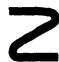
\includegraphics[keepaspectratio]{images/part001_58cd264b.jpg}}

It should be noted that the space \(\mathcal{M}(\mathrm{X};\mathbf{C})\) (or \(\mathcal{M}(\mathrm{X};\mathbf{R})\) ) itself is not necessarily complete for the vague uniform structure (TVS, II, §6, No.~7).

COROLLARY. --- If A and B are two vaguely closed subsets of \(\mathcal{M}_{+}(\mathrm{X})\) , then \(A + B\) is vaguely closed in \(\mathcal{M}_{+}(\mathrm{X})\) (hence also in \(\mathcal{M}(\mathrm{X};\mathbf{C})\) ).

This is in fact a general property of weakly complete, proper cones in locally convex spaces (TVS, II, §6, No.~8, Cor. 2 of Prop. 11).

PROPOSITION 15. --- Let H be a subset of \(\mathcal{M}(\mathrm{X};\mathbf{C})\) . The following properties are equivalent:

\begin{enumerate}
\def\labelenumi{\alph{enumi})}
\item
  H is vaguely bounded.
\item
  H is vaguely relatively compact.
\item
  H is equicontinuous.
\item
  For every compact subset K of X, there exists a number \(M_{K} \geqslant 0\) such that \(|\mu(f)| \leqslant M_{K}\|f\|\) for every measure \(\mu \in H\) and every function \(f \in \mathcal{K}(X, K; \mathbf{C})\) .
\end{enumerate}

Since \(\mathcal{K}(\mathrm{X};\mathbf{C})\) is a barreled space (No.~1, Prop. 2), the equivalence of properties a), b) and c) follows from TVS, III, §4, No.~1, Scholium.

It is clear that d) implies a). Finally, if H is equicontinuous then the set of restrictions of the measures \(\mu\in H\) to \(\mathcal{K}(X,K;\mathbf{C})\) is also equicontinuous, whence the condition d), since \(\mathcal{K}(X,K;\mathbf{C})\) is a normed space.

* We shall see in Ch. IV, §4, No.~6 that the conditions of Proposition 15 are also equivalent to the condition that, for every compact subset K of X, there exists a constant \(\mathrm{M}_{\mathrm{K}}\) such that \(|\mu|(\mathrm{K}) \leqslant \mathrm{M}_{\mathrm{K}}\) for every measure \(\mu \in \mathrm{H}\) .

COROLLARY 1. --- Let \(\nu\) be a positive measure on X; the set of measures \(\mu\) such that \(|\mu| \leqslant \nu\) is vaguely compact.

COROLLARY 2. --- The set of measures \(\mu\) such that \(\|\mu\| \leqslant a\) (a any finite number \(>0\) ) is vaguely compact.

COROLLARY 3. --- If X is compact, the set of positive measures \(\mu\) on X such that \(\|\mu\| = 1\) is vaguely compact.

For, it is the intersection of the vaguely compact set (Cor. 2) of measures such that \(\|\mu\|\leqslant1\) and the vaguely closed sets defined respectively by the relations \(\mu\geqslant0\) and \(\mu(1)=1\) (No.~8, Cor. 2 of Prop. 10).

COROLLARY 4. --- In the space \(\mathcal{M}(\mathrm{X};\mathbf{C})\) , the mapping \(\mu \mapsto \| \mu \|\) is lower semi-continuous for the vague topology.

This is an immediate consequence of Corollary 2.

\pandocbounded{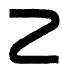
\includegraphics[keepaspectratio]{images/part001_13b41992.jpg}}

It should be noted that the mapping \(\mu \mapsto |\mu|\) of \(\mathcal{M}(\mathrm{X};\mathbf{C})\) into itself is not necessarily continuous for the vague topology (Exer. 9).

PROPOSITION 16. --- Let K be a compact subset of X, H a vaguely bounded subset of \(\mathcal{M}(\mathrm{X};\mathbf{C})\) ; then, the bilinear form \((f,\mu)\mapsto\langle f,\mu\rangle\) is continuous on \(\mathcal{K}(\mathrm{X},\mathrm{K};\mathbf{C})\times\mathrm{H}\) when \(\mathcal{K}(\mathrm{X},\mathrm{K};\mathbf{C})\) is equipped with the topology of uniform convergence and H with the vague topology.

For, there exists a number \(M \geqslant 0\) such that

\[
| \mu (f) | \leqslant \mathrm{M} \| f \|
\]

for every function \(f \in \mathcal{K}(\mathrm{X},\mathrm{K};\mathbf{C})\) and every measure \(\mu \in \mathrm{H}\) (Prop. 15). If \(\mu_0\) and \(\mu\) are two measures belonging to \(\mathrm{H}\) , \(f_0\) and \(f\) two functions in \(\mathcal{K}(\mathrm{X},\mathrm{K};\mathbf{C})\) , then

\[
\begin{array}{r l} | \mu (f) - \mu_ {0} (f _ {0}) | & = | \mu (f - f _ {0}) + \mu (f _ {0}) - \mu_ {0} (f _ {0}) | \\ & \leqslant \mathrm{M} \| f - f _ {0} \| + | \mu (f _ {0}) - \mu_ {0} (f _ {0}) |, \end{array}
\]

and the last quantity is arbitrarily small when \(\|f-f_{0}\|\) and \(|\mu(f_{0})-\mu_{0}(f_{0})|\) are, which proves the proposition.
